%!TEX root = ../swiatlow_thesis.tex
\label{chapter:susy}

\section{The Problem of the Standard Model}
\label{chapter:susy:problems}

It is somewhat incongruous to say that the SM has problems after describing the degree of its success in Chapter~\ref{chapter:sm}, but there are clear tensions in the model which point to signs of potential new extensions. The following chapter describe some of these shortcomings, and introduces an extension called \textit{supersymmetry} that alleviates some of these issues\cite{Miyazawa:1966,Ramond:1971gb,Golfand:1971iw,Neveu:1971rx,Neveu:1971iv,Gervais:1971ji,Volkov:1973ix,Wess:1973kz,Wess:1974tw}. The experimental consequences of supersymmetry are then discussed, and the landscape of searches at particle colliders is evaluated.

\subsection{The Pursuit of Beauty, or Naturalness}
\label{chapter:susy:problems:naturalness}
The process of developing a fundamental theory of nature is intended to be simplifying: for example, the development of the parton model and QCD simplified the eight-fold way and the complicated sea of hadrons  that came before it~\cite{Politzer:1973fx,Gross:1973ju,Gross:1973id}. The core of this simplification was the realization of a symmetry--- the $SU(3)$ of color--- which reduced a complicated system to a more simple one. There is an element to this that a physicist might call beautiful: the realization of an underlying simple pattern which explains something complicated. In that sense, there should be very few accidents in a theory: there should be a \textit{reason} for things to be the way they are. For example, there are no accidental, or ad-hoc terms in a Lagrangian: we include all relevant terms allowed by the symmetry groups, and derive the consequences. The symmetry groups are the reason that the Lagrangians look the way they do \cite{schwartz}.

In this same sense, constants in the theory can be arbitrary, but requiring them to be \textit{arbitrarily precise} is something of an aesthetic problem: the theory should not care if the mass of the up or down quark were different by $50\%$, for example. However, there is exactly one such finely tuned mass in the Standard Model: $m_h$, the mass of the Higgs boson. 

As discussed in Section~\ref{chapter:sm:qcd:freedom}, higher-order terms caused by loop diagrams induce corrections to parameters, such as masses and coupling constants, through the process of renormalization. The Higgs boson's mass is not immune, and since the Higgs couples to all particles (except gluons) via either gauge coupling terms or the Yukawa couplings to matter, all of these particles create loops which correct the Higgs mass. Because it has the largest coupling, the loop involving the top quark--- pictured in Figure~\ref{fig:susy:higgs-loop}---  has the largest contribution out of all these terms~\cite{Martin1997}. The correction goes as:
%
\begin{equation}
\Delta m_H^2 \approx - \frac{|y_T|^2}{8\pi^2}\Lambda_\mathrm{UV}^2 + \ldots
\end{equation}
%
where $y_T$ is the top Yukawa coupling, and $\Lambda_\mathrm{UV}$ is the UV cutoff of the theory~\cite{Martin1997}. This correction grows quadratically with the cut-off scale: if the SM is the only theory of nature up to the Planck scale (where quantum gravity takes effect, thereby signficantly changing the appropriate physical description), then the correction is proportional to $M_\mathrm{Planck}^2$. The observed Higgs boson has a mass of 125 GeV~\cite{CombinedHiggs}, which is quite far from $M_\mathrm{Planck} = 1.22\times 10^{19}$~GeV: the only way to reconcile the measurement with the observation, is to set $m_0$, the bare Higgs mass before corrections, to a \textit{precise} value such that $m_0$ and $\Delta m_H^2$ cancel perfectly to 125 GeV. Thus, the SM requires the bare mass to be  defined to 1 part in $10^{19}$, a value so precisely specified that it seems unlikely to have arisen by chance. 

%%%%%%%%%%%%%%%%

\begin{figure}
\centering
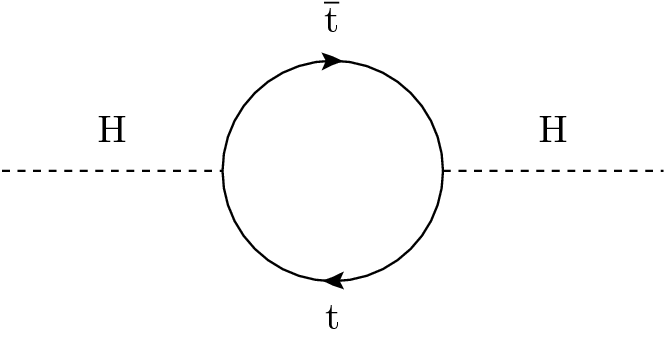
\includegraphics[width=0.7\textwidth]{higgs-loop.png}
\label{fig:susy:higgs-loop}
\caption{An example of a loop diagram which renormalizes the Higgs mass. Courtesy of PyFeyn.}
\end{figure}

%%%%%%%%%%%%%%%%  

Thus, the mass of the Higgs boson is not like that of other constants in the theory. Particles such as quarks and leptons do not receive quantum corrections to their masses, so there is no expectation for their masses; moreover, the observed mass of the Higgs is substantially outside of the expected range (around the Planck scale).  The SM's solution to this issue--- a precise cancelling of terms--- has an aesthetic penalty: there is no \textit{reason} for this cancellation in the SM, only blind luck. Physicists say that this kind of solution lacks \textit{naturalness}: there is no underlying symmetry or simplification to explain it, and only a very particular number.



\subsection{Unification}

Another aesthetic criticism of the SM lies in its separation of forces. The electroweak model is seen as particularly elegant because the electroweak symmetry, though broken at low energies by the Higgs mechanism, provides a unifying structure to two initially disparate forces (electomagnetism and the weak force). One natural question is whether some higher symmetry group unifies all the SM forces, and not just the electroweak. Figure~\ref{fig:susy:couplings_sm} shows the strength of the coupling constants in the SM as a function of the energy scale $\mu$: while they nearly intersect--- implying a potential for unification--- they just barely miss~\cite{susypheno}.


%%%%%%%%%%%%%%%%

\begin{figure}
\centering
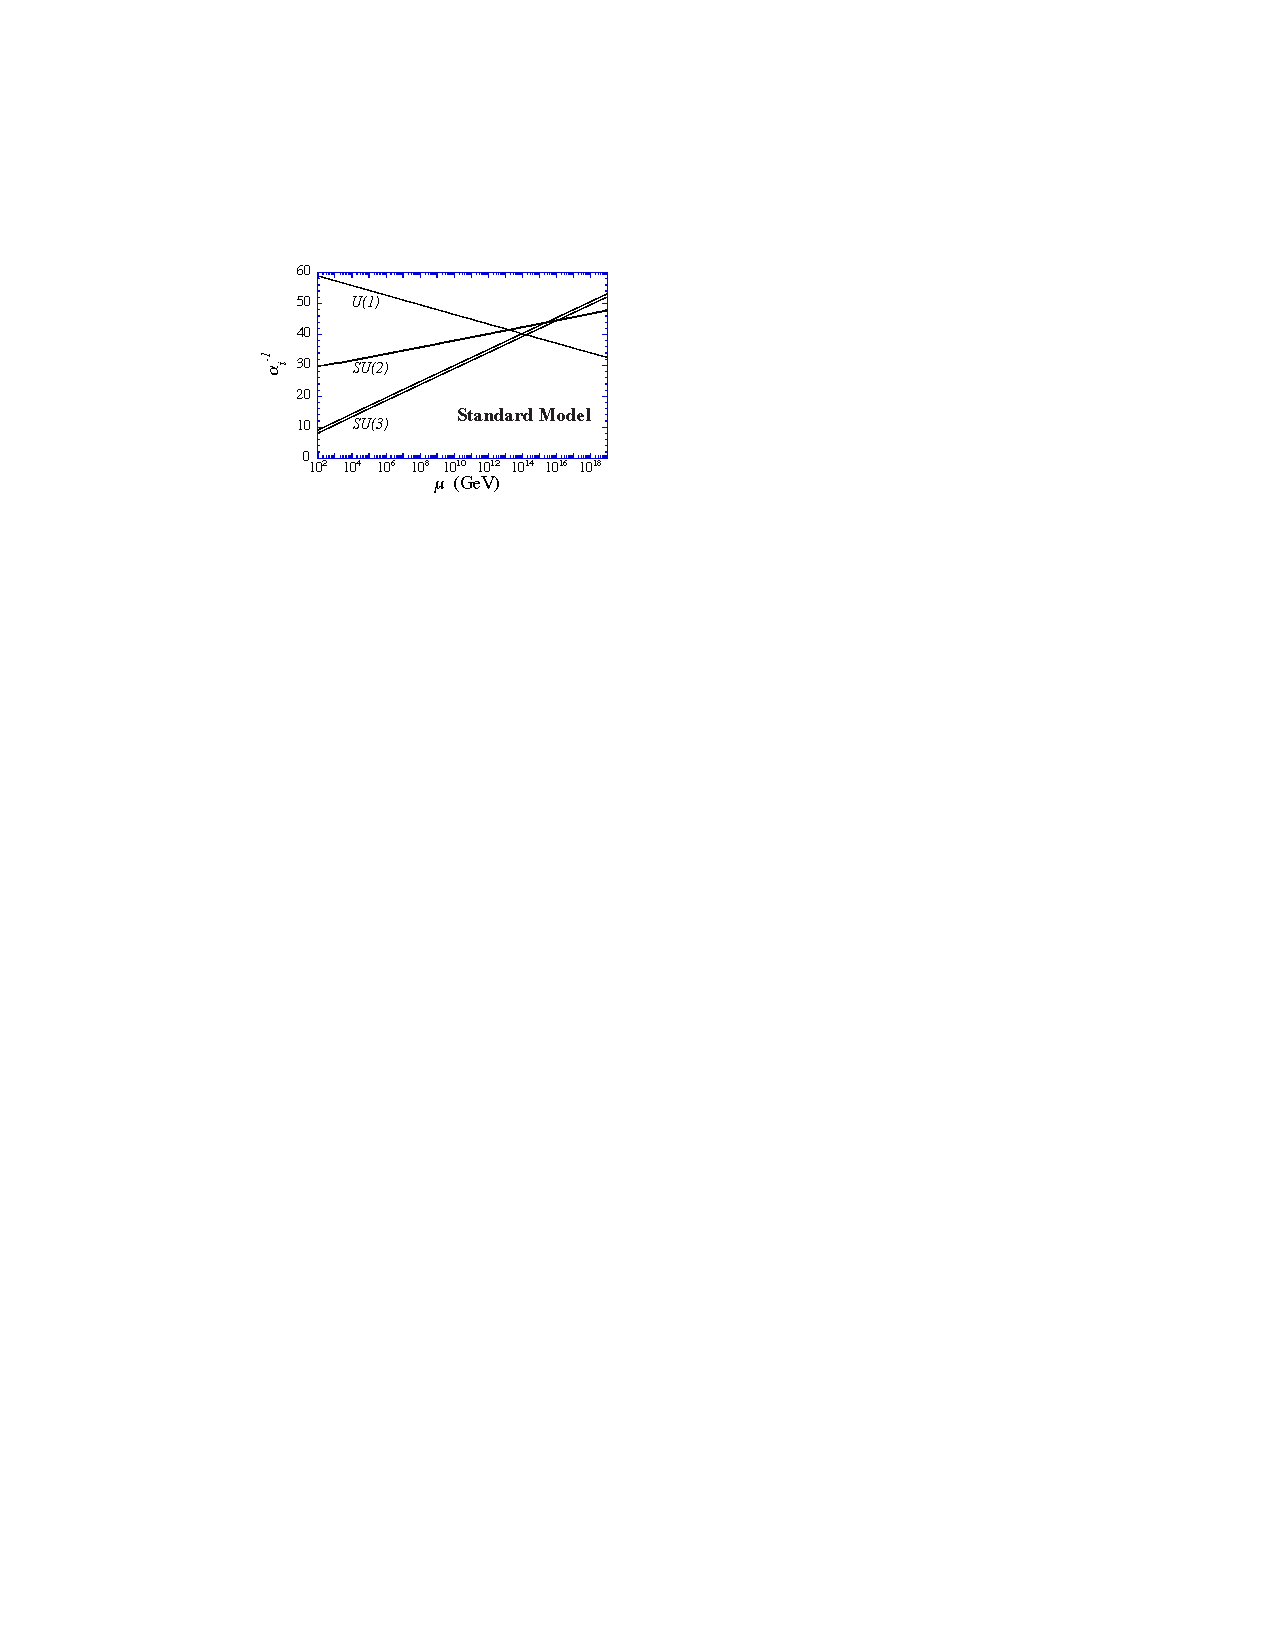
\includegraphics[width=0.7\textwidth]{couplings_sm.pdf}
\label{fig:susy:couplings_sm}
\caption{The evolution of the strength of the coupling constants of the three symmetry groups of the SM. While they come close to unifying, they never cross the same point. Figure from \cite{susypheno}.}
\end{figure}

%%%%%%%%%%%%%%%%  

While unification is certainly not \textit{required}, it seems like a shame that such an opportunity would be missed. Moreover, such a unification could explain the unexplained relationships in charge quantization between quarks and leptons~\cite{SUSYUnification}. Replacing two distinct forces with one overarching theory governed by one simple symmetry group would be a substantial simplification of the underlying model.

\subsection{Dark Matter}


One final motivation for the existence of physics beyond the SM is based on firm experimental ground: this is the presence of dark matter in the universe~\cite{Jungman}. Dark matter refers to the presence of matter that is inferred from observations of gravitational effects in the galaxy and beyond: these measurements indicate that there must be some source of mass, making up approximately 85\% of the mass of the universe, which does not emit light. Figure~\ref{fig:susy:bullet} shows one of the strongest observational pieces of evidence: the Bullet Cluster~\cite{Tucker:1998tp,Markevitch:2003at}. Two clusters of galaxies are passing through each other in this figure:; the blue area indicates regions with a large number of stars, while the purple area indicates areas with a large concentration gas which slowed down due to the collisions of the clusters. This gas contains most of the visible matter in the clusters, but gravitational lensing measurements (which study how light coming from behind the clusters bends) indicate that most of the mass occurs with the stars instead. This implies that another type of matter also passed through the collision along with the stars, and is hypothesized to be Dark Matter. Many other observations, such as the distributions of rotational speeds in sprial galaxies~\cite{Rubin}, the simulations of large scale structures in the universe~\cite{Springel:2005nw}, and measurements of the cosmic microwave background radiation~\cite{Ade:2015xua}, yield a consistent story of a significant amount of unaccountable matter.


%%%%%%%%%%%%%%%%

\begin{figure}
\centering
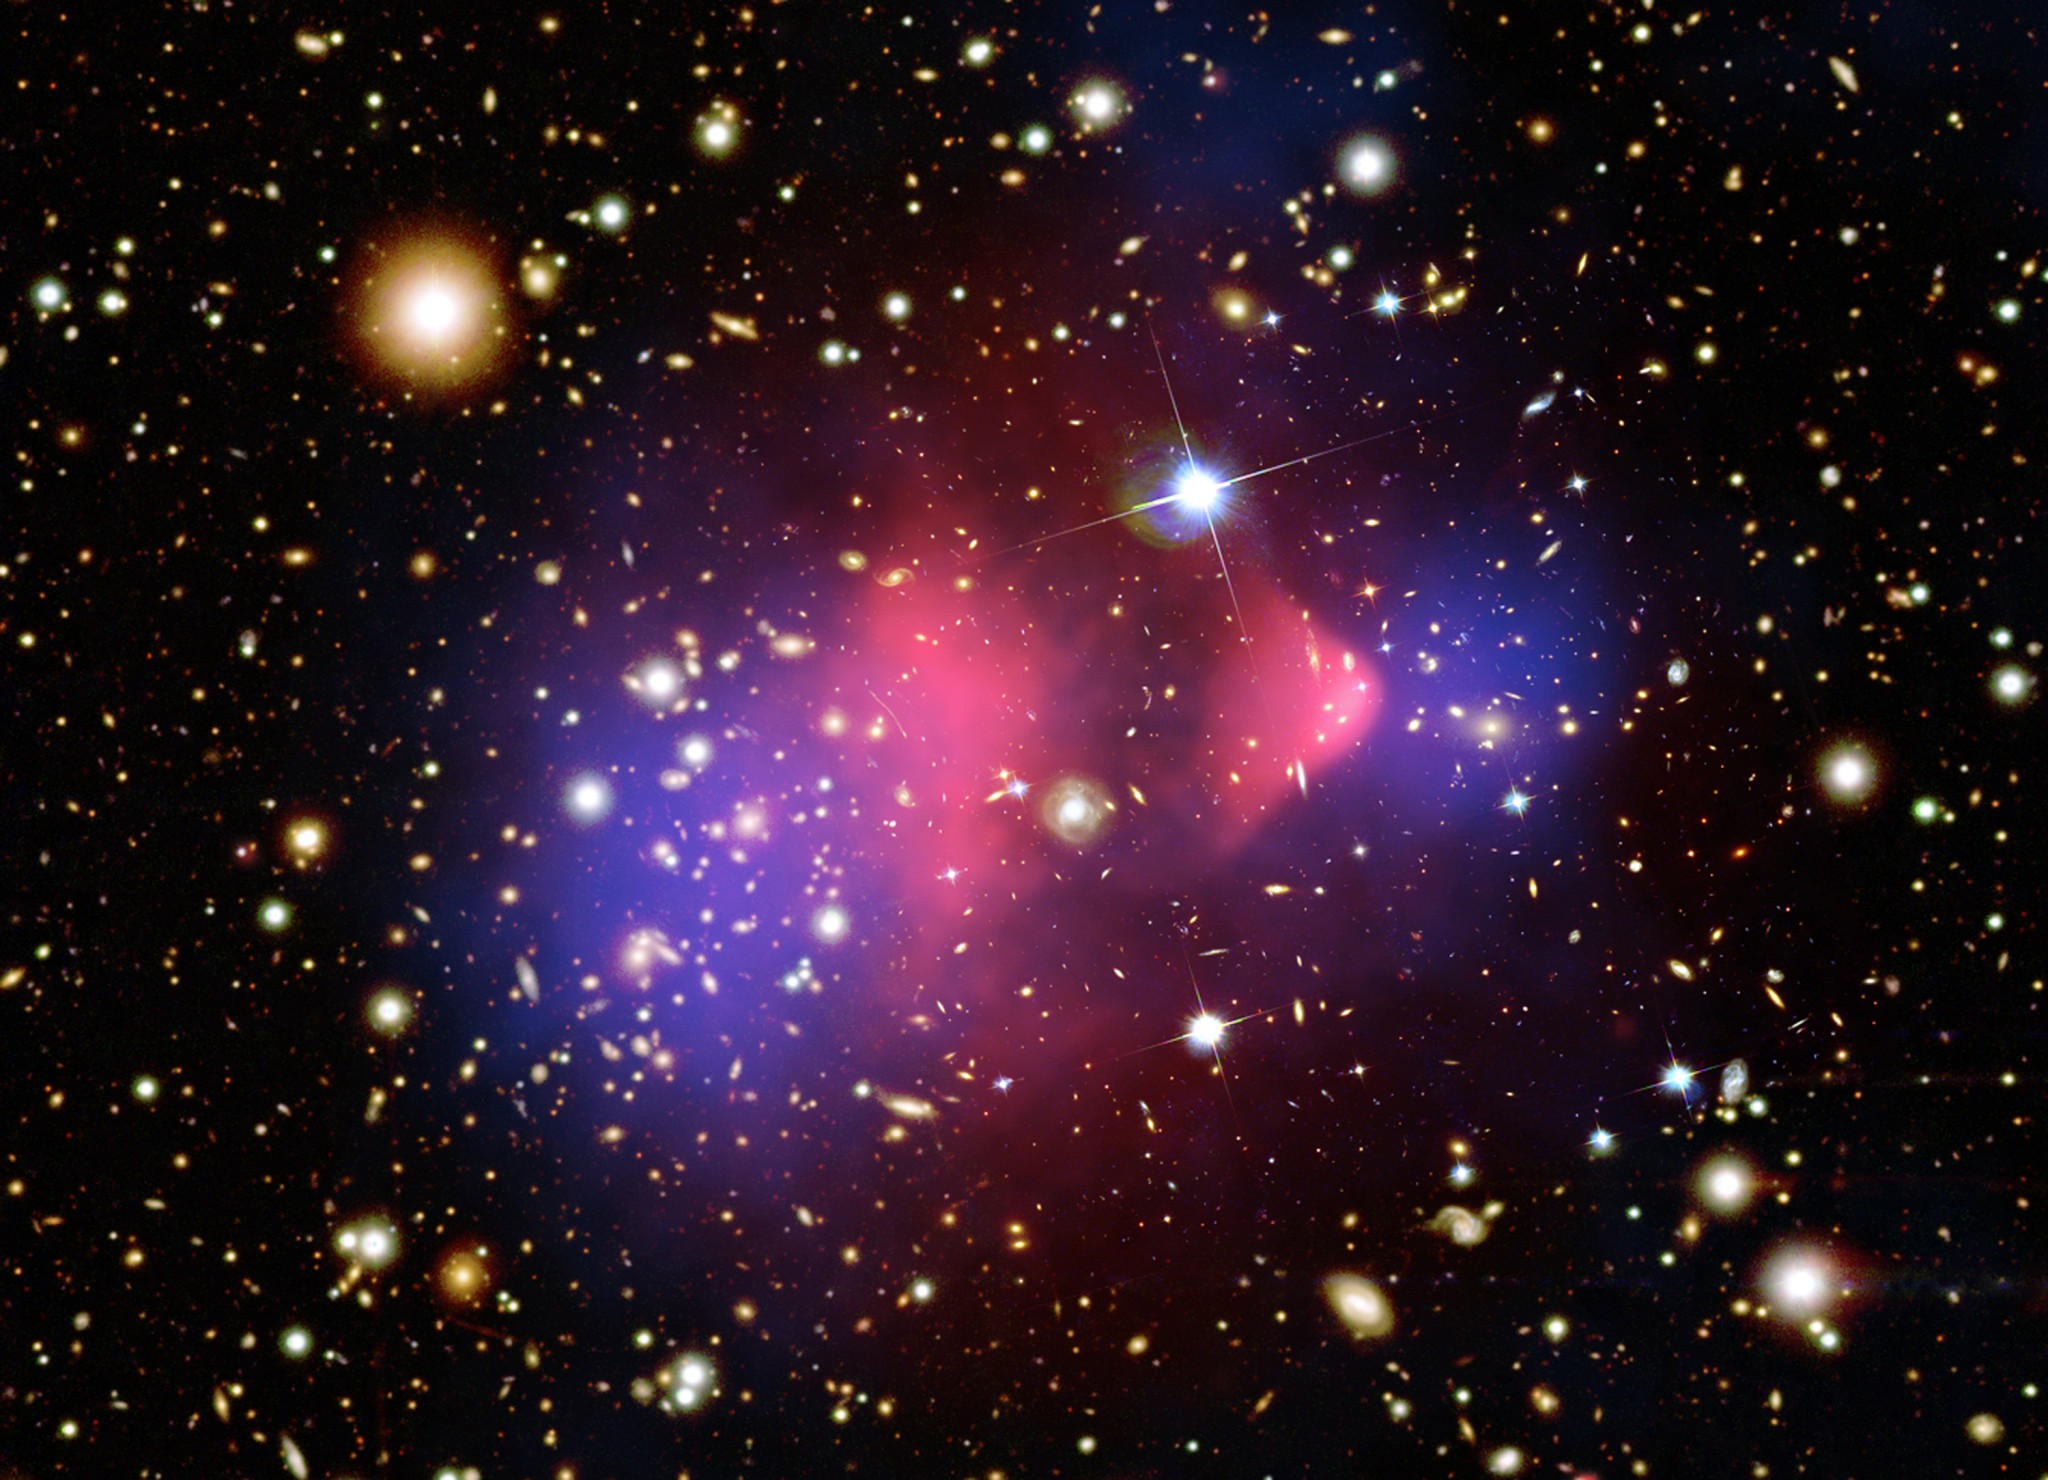
\includegraphics[width=0.7\textwidth]{bullet}
\label{fig:susy:bullet}
\caption{A false-color image of the Bullet Cluster, two colliding clusters of galaxies. The purple coloring indicates the stronger presence of gravitionally inferred mass, while the blue coloring indicates the stronger presence of electromagnetically observed mass.}
\end{figure}

%%%%%%%%%%%%%%%%  

Since dark matter is interacting gravitionally, and all other matter we are familiar with has come in the form of particles, it is natural to ask what particle dark matter possibly could be. There is one matter particle in the SM which interacts weakly and is therefore a potential candidate: these are the neutrinos, $\nu$. Unfortunately, their vanishingly small mass means that they would not be very strongly gravitionally interacting either, while many observations (such as the mass of galaxies) suggest that dark matter can ``clump'' together. This means that there are no candidates in the SM for dark matter, and we must look beyond the standard model to understand the nature of dark matter~\cite{Jungman}.


\section{Supersymmetry: The Solution?}


These three shortcomings of the SM motivate the need for new theories--- but it turns out that there is a way to solve all three problems at once. The solution is to introduce a new symmetry to the model which creates a boson for every fermion, and vice versa. This theory, called \textit{supersymmetry}, or SUSY, symmetrizes the distinction between matter and interactions in the SM, and creates a framework for describing all particles--- fermions and bosons--- simultaneously~\cite{Martin1997,susypheno}.

%new particles

\subsection{Developing SUSY} 

\label{chapter:susy:susy:developing}

Writing down the Lagrangain for SUSY requires us to write it in a form that maintains the symmetry and requires some new notation. An unbroken supersymmetric theory is most naturally written in terms of supermultiplets (combinations of fermions and bosons) to maintain the symmetry explicitly~\cite{Jungman}. 

Before we go further, there is another type of well-motivated symmetry most versions of SUSY entail: $R$-parity, or matter symmetry\cite{Jungman}. $R$ parity can be defined as $R = (-1)^{3(B-L)+2S}$ where $B$ is baryon number, $L$ is lepton number, and $S$ is spin. Thus, $R = 1$ for SM particles and $R = -1$ for SUSY particles. The preservation of $R$ parity is critical to generating a SUSY dark matter candidate: if it were not preserved, SUSY particles with masses $\mathcal{O}(\mathrm{GeV})$ could decay to SM particles, and no stable lightest supersymmetric particle (LSP) would exist. The Lagrangian for the MSSM that we are considering, in the spirit of the simplest, most minimal theory, will thus require invariance under SUSY transformations, R parity, and renormalizability for all terms \cite{Jungman}. Note that the $R$-parity requirement is not strictly necessary, and we will consider alternatives in detail in Section~\ref{chapter:susy:r}.

%cite georgi at some point? why not

For completeness, let us now write out an example of a superfield which enters the Lagrangian. The relationships between terms are given as polynomials in abstract spinor symbols $\theta_\alpha$ and $\overline{\theta}_{\dot{\alpha}}$ which represent the superspace coordinates. A generic superfield will thus be of the form \cite{Jungman}:
\begin{align}
  \Phi(x, \theta_\alpha, \overline{\theta}_{\dot{\alpha}}) &= f(x) + \theta_\alpha \psi^\alpha(x) + \overline{\theta}_{\dot{\alpha}} \chi^{\dot{\alpha}} + \theta_\alpha \theta^\alpha m(x) + \overline{\theta}_{\dot{\alpha}} \overline{\theta}^{\dot{\alpha}} + \theta_\alpha \s^{\mu \alpha \dot{\alpha}} \overline{\theta}_{\dot{\alpha}} v_\mu(x) \nonumber\\
  &\quad + \theta_\alpha \theta^\alpha \overline{\theta}_{\dot{\alpha}} \overline{X}^{\dot{\alpha}}(x) + \overline{\theta}_{\dot{\alpha}} \overline{\theta}^{\dot{\alpha}} \theta_\alpha \phi^\alpha (x) + \theta_\alpha \theta^\alpha \overline{\theta}_{\dot{\alpha}} \overline{\theta}^{\dot{\alpha}}\mathrm{d}(x)
\end{align}
As expected, we have spinor, vector, and scalar fields. Some of these will be non-dynamical and can be integrated out using the equations of motion; the remaining terms will be the SM particles and their SUSY partners. Using the integration definitions for the Grassman-valued $\theta$'s, and putting together standard renormalizable action terms, we have a generic action of \cite{Jungman}:
\begin{align}
  S = \int d^4 x\left[ \int d^2\theta d^2 \theta \Phi^\dagger \Phi + \int d^2\theta \left( \lambda \Phi + m \Phi \Phi + \kappa \Phi \Phi \Phi \right) \right]
\end{align}
The first term is the standard kinetic term; the second term is the superpotential. The question now is what superfields to actually include. Inspired by the Standard Model choices, we want to include quark/lepton superfields of the form $\hat{L}_{Li}$, $\hat{e}_{Ri}$, $\hat{Q}_{Li}$, $\hat{d}_{Ri}$, $\hat{u}_{Ri}$, where $i$ is a generational index and $L$ or $R$ indicate handedness. Additionally, two Higgs superfields are required, $\hat{H}_1$ and $\hat{H}_2$, to give mass to all particles. \footnote{One Higgs is not sufficient, as traditionally down-type quarks acquire mass from a $H^c = i \sigma_2 H^*$ type interaction, but the $H^*$ field is not allowed in the supersymmetric Lagrangian. Another Higgs particle is thus required to give mass to down-type quarks and the other particles that $H^c$ would normally have interacted with.} Note that hats indicate superfields, as opposed to normal fields. Additionally, we should add on the vector superfields that of the U(1)$_Y\times$SU(2)$_W\times$SU(3)$_c$ gauge symmetry: $\hat{B}$, $\hat{W}^a$, and $\hat{G}^a$ \cite{Jungman}.

With these fields, and the general form of an acceptable action written above, we can assemble the supersymmetric Lagrangian:
\begin{align}
  \mathcal{L}_s = \mathcal{L}_\mathrm{kinetic} + \int d^2\theta \left( -\mu \hat{H}_1 \hat{H}_2 + \hat{H}_1 h_c^{ij}\hat{L}_{Li} \hat{e}_{Rj} + \hat{H}_1 h^{ij}_d \hat{Q}_{Li} \hat{d}_{Rj} - \hat{H}_2 h^{ij}_u \hat{Q}_{Li} \hat{u}_{Rj} \right)
\end{align}
where the term being integrated over $\theta$ is the superpotential $\mathcal{W}$. This theory is now manifestly supersymmetric, as it contains only superfields invariant under supersymmetry. 

Of course, it is understood that at energies below a scale $E_{sb}$, spontaneous symmetry breaking occurs and supersymmetry is broken. But, it is important that it breaks in such a way that the softened ultraviolet behavior of the radiative corrections is preserved. In particular, the most general gauge-invariant terms that break supersymmetry but respect our other conditions are \cite{Jungman}:
\begin{align}
  \mathcal{L}_\mathrm{soft} = &-m_1^2 |H_1|^2 - m_2^2 |H_2|^2 - m_{12}^2 \left( H_1 H_2 + H_1^* H_2^* \right) - \tilde{Q}_{Li}^\dagger M_{\tilde{Q} ij}^2 \tilde{Q}_{Lj} - \tilde{u}^\dagger_{Ri} M^2_{\tilde{u} i j} \tilde{u}_{Rj}\nonumber\\
  &-\tilde{d}_{Ri}^\dagger M^2_{\tilde{d} i j} \tilde{d}_{Rj} -\hat{L}^\dagger_{Li} M^2_{\tilde{L} ij} \tilde{L}_{Lj} - \tilde{e}^*_{Ri} M^2_{\tilde{e} ij} \tilde{e}_{Rj} + H_2 \tilde{Q}_{Li}(h_u A_u)_{ij} \tilde{u}_{Rj} -H_1 \tilde{Q}_{Li} (h_d A_d)_{ij} \tilde{d}_{Rj}\nonumber\\
  &-H_1 \tilde{L}_{Li} (h_e A_e)_{ij} \tilde{e}_{Rj} - \frac{1}{2} \left[ M_1 \overline{\tilde{B}} \tilde{B} + M_2 \overline{\tilde{W}}^a \overline{W}^a + M_3 \overline{\tilde{G}}^a \tilde{G}^a \right]
\end{align}
where $A$ terms are mass matrices in flavor space, and the rest of the definitions are soft mass terms. The fields here are no longer superfields, and the $\sim$ indicate superpartners of Standard Model fields. Combined with $\mathcal{L}_s$, this gives a full description of the particles and fields of a broken supersymmetric theory, but the superfields from $\mathcal{L}_s$ remain.


\subsection{The Particles of SUSY}

With the SUSY Lagrangian defined, we can now assess the actual particle content. The naming scheme is rather whimsical, but helpfully makes explicit the connections to existing SM particles. Supersymmetric fermions (i.e., those particles which have boson partners in the SM) take the name of their boson partner with `ino' appended: hence, gluinos $\tilde{g}$. Supersymmetric bosons take the name of their partner, but `s' is preprended: hence, staus $\tilde{\tau}$ or stops $\tilde{t}$. The $\sim$ character always indicates that the particle is the supersymmetric partner of the corresponding SM particle.

For many of the particles--- particularly those with significant Yukawa couplings to the Higgs sector--- it is not possible to simultaneously diagonalize the gauge eigenstates (i.e., the interaction eigenstates) with the mass eigenstates. 

For example, the supersymmetric partners of the electroweak gauge bosons and higgs bosons are the Wino, Bino, and Higgsinos. The neutral gauginos ($\tilde{B}$ and $\tilde{W}^0$) and the neutral Higginos ($\tilde{H}^0_d$ and $\tilde{H}^0_u$) are coupled together in a mixed mass matrix,  written in the $\tilde{B}-\tilde{W}^0-\tilde{H}_u^0-\tilde{H}_u^0$ basis\cite{Martin1997}:
\begin{align}
  M_\mathrm{neut}=
\left(
\begin{array}{cccc}
 M_1 & 0 & -c_{\beta } m_z s_w &
   m_z s_{\beta } s_w \\
 0 & M_2 & c_{\beta } c_w m_z &
   -c_w m_z s_{\beta } \\
 -c_{\beta } m_z s_w & c_{\beta }
   c_w m_z & 0 & -\mu  \\
 m_z s_{\beta } s_w & -c_w m_z
   s_{\beta } & -\mu  & 0
\end{array}
\right)  \label{eqn:massx}
\end{align}
%
where the $s$ and $c$ refer to sines and cosines of the mixing angles $\theta_W$ and $\beta$, which are reparametrizations of the vev terms which broke the electroweak symmetry and introduced masses to the gauginos and higgsinos. Diagonalizing this matrix allows us to form the neutralinos: 4 mixtures of the neutral gauginos and higginos, with $m_{\neutFour} > m_{\neutThree} > m_{\neutTwo} > m_{\neutOne}$. A similar process mixes the charged gauginos ($\tilde{W}^\pm$) and the charged Higgsinos $\tilde{H}^+_u$ and $\tilde{H}^-_d$ into the mass eigenstates called charginos, denoted $\tilde{C}^\pm_1$ and $\tilde{C}^\pm_2$. The neutralinos will play an important role in some of the phenomonology later described~\cite{Martin1997}.

Gluinos $\tilde{g}$ are comparatively simple: as they are completely uninvolved in electroweak symmetry breaking, there is no complicated relationship between gauge eigenstates and mass eigenstates, as they are able to share the same basis. The large color charge of the gluino ends up important consequences; these will be discussed shortly.

Squarks and sleptons are once again more complicated: in principle the mass matrix should be obtained by diagonalizing a $6\times6$ matrix which couples the up-type squarks to each other ($\tilde{u}_L$, $\tilde{c}_L$, $\tilde{t}_L$, $\tilde{u}_R$, $\tilde{c}_R$, $\tilde{t}_R$), a similar one for the the down-type squarks to each other ($\tilde{d}_L$, $\tilde{s}_L$, $\tilde{b}_L$, $\tilde{d}_R$, $\tilde{s}_R$, $\tilde{b}_R$), a similar one for the sleptons, and a $3\times3$ one for the sneutrinos. Typically, flavor-blind soft symmetry breaking terms\footnote{Very often the soft symmetry breaking terms are introduced as flavor-independent because of the strong constraints on flavor physics from precision measurements at $B$-factories and other sources.} mean that mixing amongst the first two generations is very small; in turn, this means that the gauge and mass eigenstates are the same (to first order in this small mixing). The third generation is more complicated, and can have significant mixing terms~\cite{Martin1997}. The mixing matrix from gauge eigenstates to max eigenstates for the stop, for example, is:
%
\begin{align}
\left(\begin{array}{c}
\tilde{t}_1\\
\tilde{t}_2
\end{array} \right) = 
\left( \begin{array}{cc}
c_{\tilde{t}} & -s_{\tilde{t}}^* \\
s_{\tilde{t}} & c_{\tilde{t}}
\end{array}\right)
\left(\begin{array}{c}
\tilde{t}_L\\
\tilde{t}_R
\end{array} \right)
\end{align}
%
where $c_{\tilde{t}}$ and $s_{\tilde{t}}$ are mixing angles composed from various components of the Yukawa couplings and soft breaking terms which couple the left and right stop squarks together~\cite{Martin1997}. The sbottoms and staus have similar matrices defined.

Table~\ref{fig:susy:susy_particles} shows a summary of these various SUSY particles and their eigenstates. Though the theory at energies above the SUSY-breaking scale is quite simple, the broken Lagrangian at low energy has more than double the particle content compared to the SM.


%%%%%%%%%%%%%%%%

\begin{table}
\centering
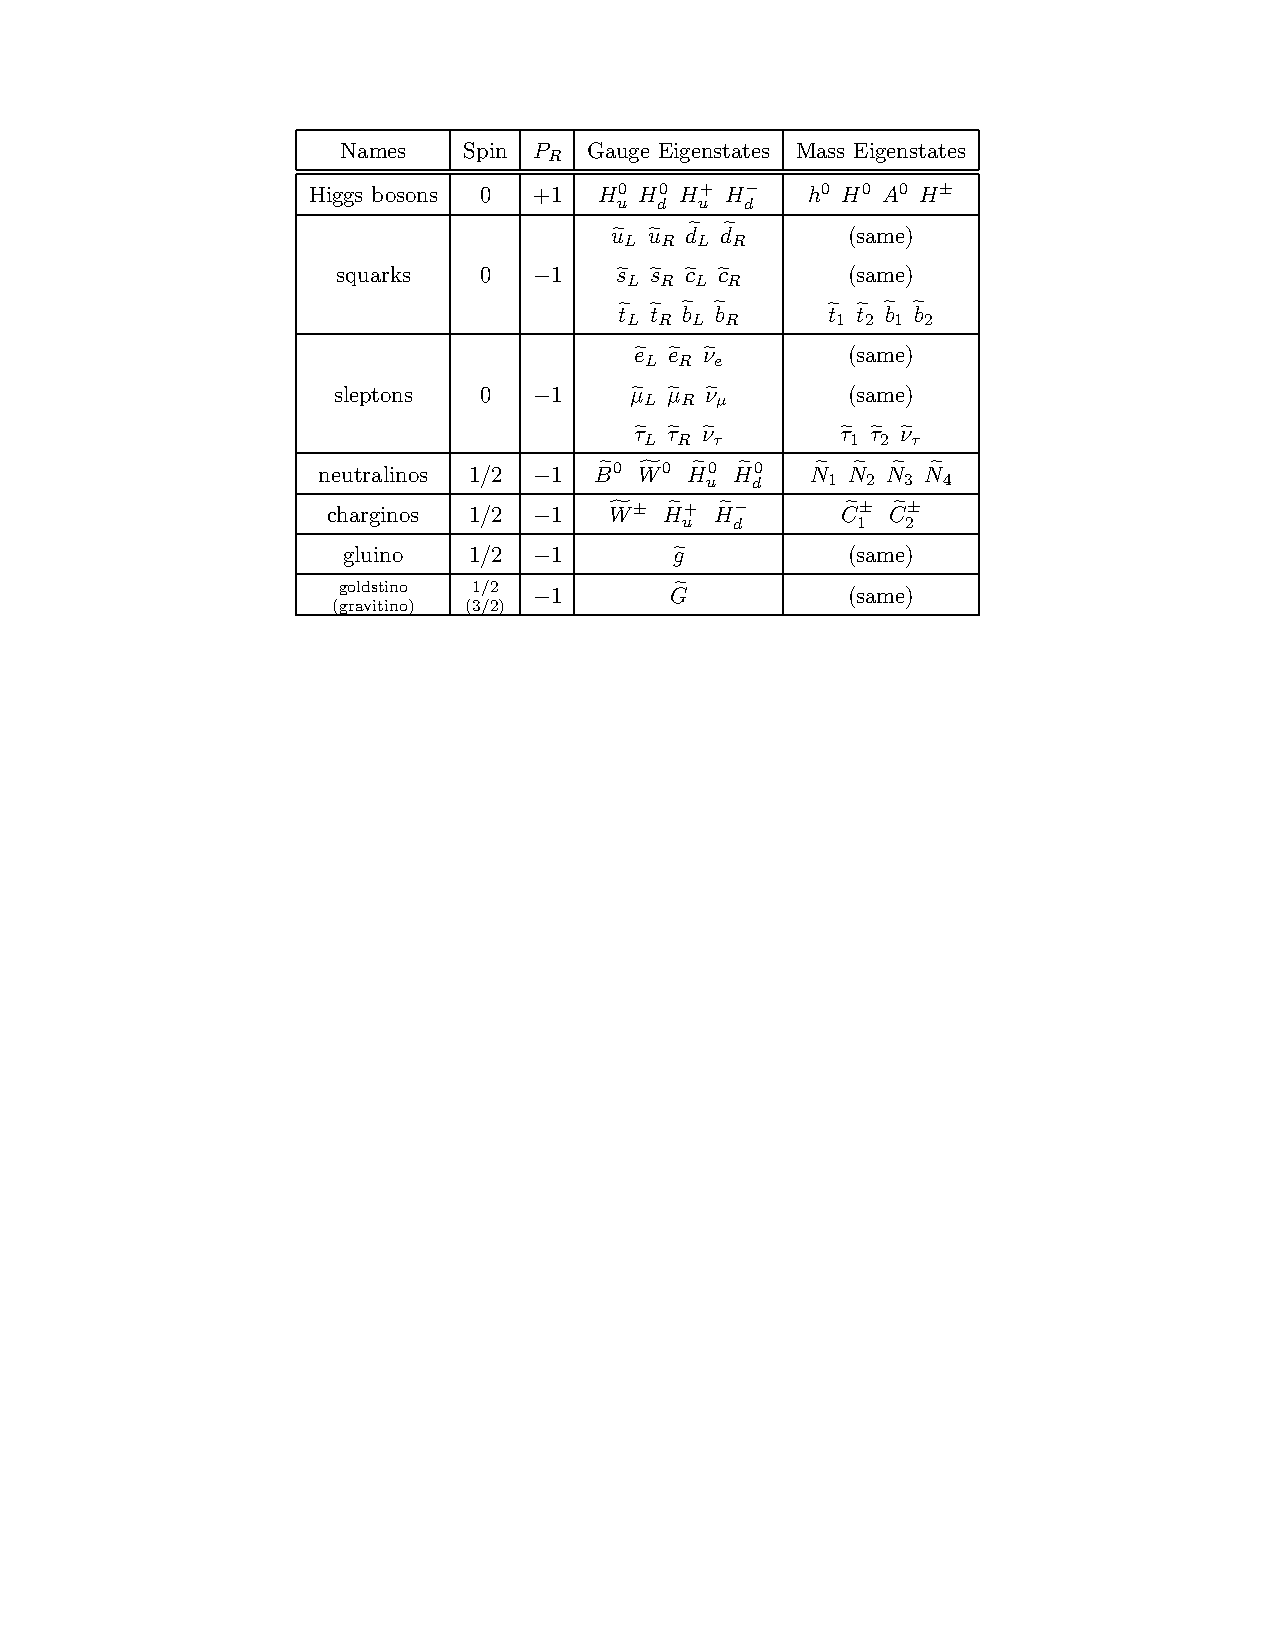
\includegraphics[width=0.7\textwidth]{susy_particles}
\label{fig:susy:susy_particles}
\caption{A table of the various SUSY particles in the MSSM, from~\cite{Martin1997}.}
\end{table}

%%%%%%%%%%%%%%%%  


% From astrophysics observations, we know that a candidate WIMP must be heavy and neutral, so we are interested in the SUSY particles which fit this criterea. In particular, what matters to us is the particular linear combination of $\tilde{B}$, $\tilde{W}^3$, $\tilde{H}_1^0$, and $\tilde{H}_2^0$. The superpotential introduces quadratic couplings between the these four fields when the supersymmetry is broken and after the Higgs particles have acquired a vev and spontaneously broken the remaining symmetry. In particular, the couplings are defined by the mass matrix:
% \begin{align}
%   M_\mathrm{neut}=
% \left(
% \begin{array}{cccc}
%  M_1 & 0 & -c_{\beta } m_z s_w &
%    m_z s_{\beta } s_w \\
%  0 & M_2 & c_{\beta } c_w m_z &
%    -c_w m_z s_{\beta } \\
%  -c_{\beta } m_z s_w & c_{\beta }
%    c_w m_z & 0 & -\mu  \\
%  m_z s_{\beta } s_w & -c_w m_z
%    s_{\beta } & -\mu  & 0
% \end{array}
% \right)  \label{eqn:massx}
% \end{align}
% This matrix is in the $\tilde{B}-\tilde{W}^3-\tilde{H}_1^0-\tilde{H}_2^0$ basis, and diagonalized by a transformation: $M_\mathrm{neut}^\mathrm{diag} = N^\dagger M_\mathrm{neut} N$, where we expect $N$ to appear as a mixing matrix in neutralino interaction terms. From the diagonalization of this matrix, 4 mass eigenstates appear, labelled $\chi_m^0$ with $m\in\{1,2,3,4\}$ \cite{Jungman}. Heavy neutralinos will decay down the spectrum to the lightest.

% However, it is not immediately clear what makes the $\chi$ a good candidate to be the LSP, as other superparticles could be lighter.  But the Higgsinos have Yukawa couplings to other particles, and in particular the large contributions of top loops lead Yukawa couplings to run negative in low energies \cite[p.~80]{Martin1997}. While the exact values of the runnings are of course very model dependent, Figure~\ref{fig:mass-run} gives an example of this sort of running \cite[p.~80]{Martin1997}. The dominant effect on $M_1$ is indeed the top-Yukawa coupling which pulls down the mass below others, whereas SU(3) couplings pull the mass of squarks much higher, for example \cite[p.~81]{Martin1997}.



% Writing out the mixing parameters explicitly, we thus have:
% \begin{align}
%   \chi = N_{10}^* \tilde{B} + N_{20}^* \tilde{W}^3 + N_{30}^* \tilde{H}_1^0 + N_{40}^* \tilde{H}_2^0
% \end{align}
% where $N$ is the neutralino mixing matrix which arises from the diagonalization of the mass matrix in eqn. \ref{eqn:massx}. 

% We have shown, then, that $MSSM$ produces a wide variety of new particles when we write down an initial unbroken Lagrangian using superfields that must be invariant under SUSY transformations. Soft, explicit breaking of the supersymmetry introduces additional couplings; combined with the couplings in the superfields themselves, we generate a mass matrix $M_\mathrm{neut}$ which couples the Higgsinos, Bino, and Wino fields. Diagonalizing this matrix leads to new mass eigenstates, the neutralinos $\chi$. The lightest of these is a good candidate to be the LSP, as RG running of masses makes most other particles much heavier at energies below the supersymmetry breaking scale.



\subsection{Fixing Naturalness}

We began exploring SUSY to fix the holes of the Standard Model. The most pressing of these\footnote{Obviously this is a matter of personal taste, though certainly to me this is the largest concern with the Standard Model as it stands.} was the naturalness issue, where diverging top loops in the Higgs boson mass renormalization required incredibly precise fine-tuning to cancel, as described in Section~\ref{chapter:susy:problems:naturalness}. How does SUSY solve this issue?

%%%%%%%%%%%%%%%%

\begin{figure}
\centering
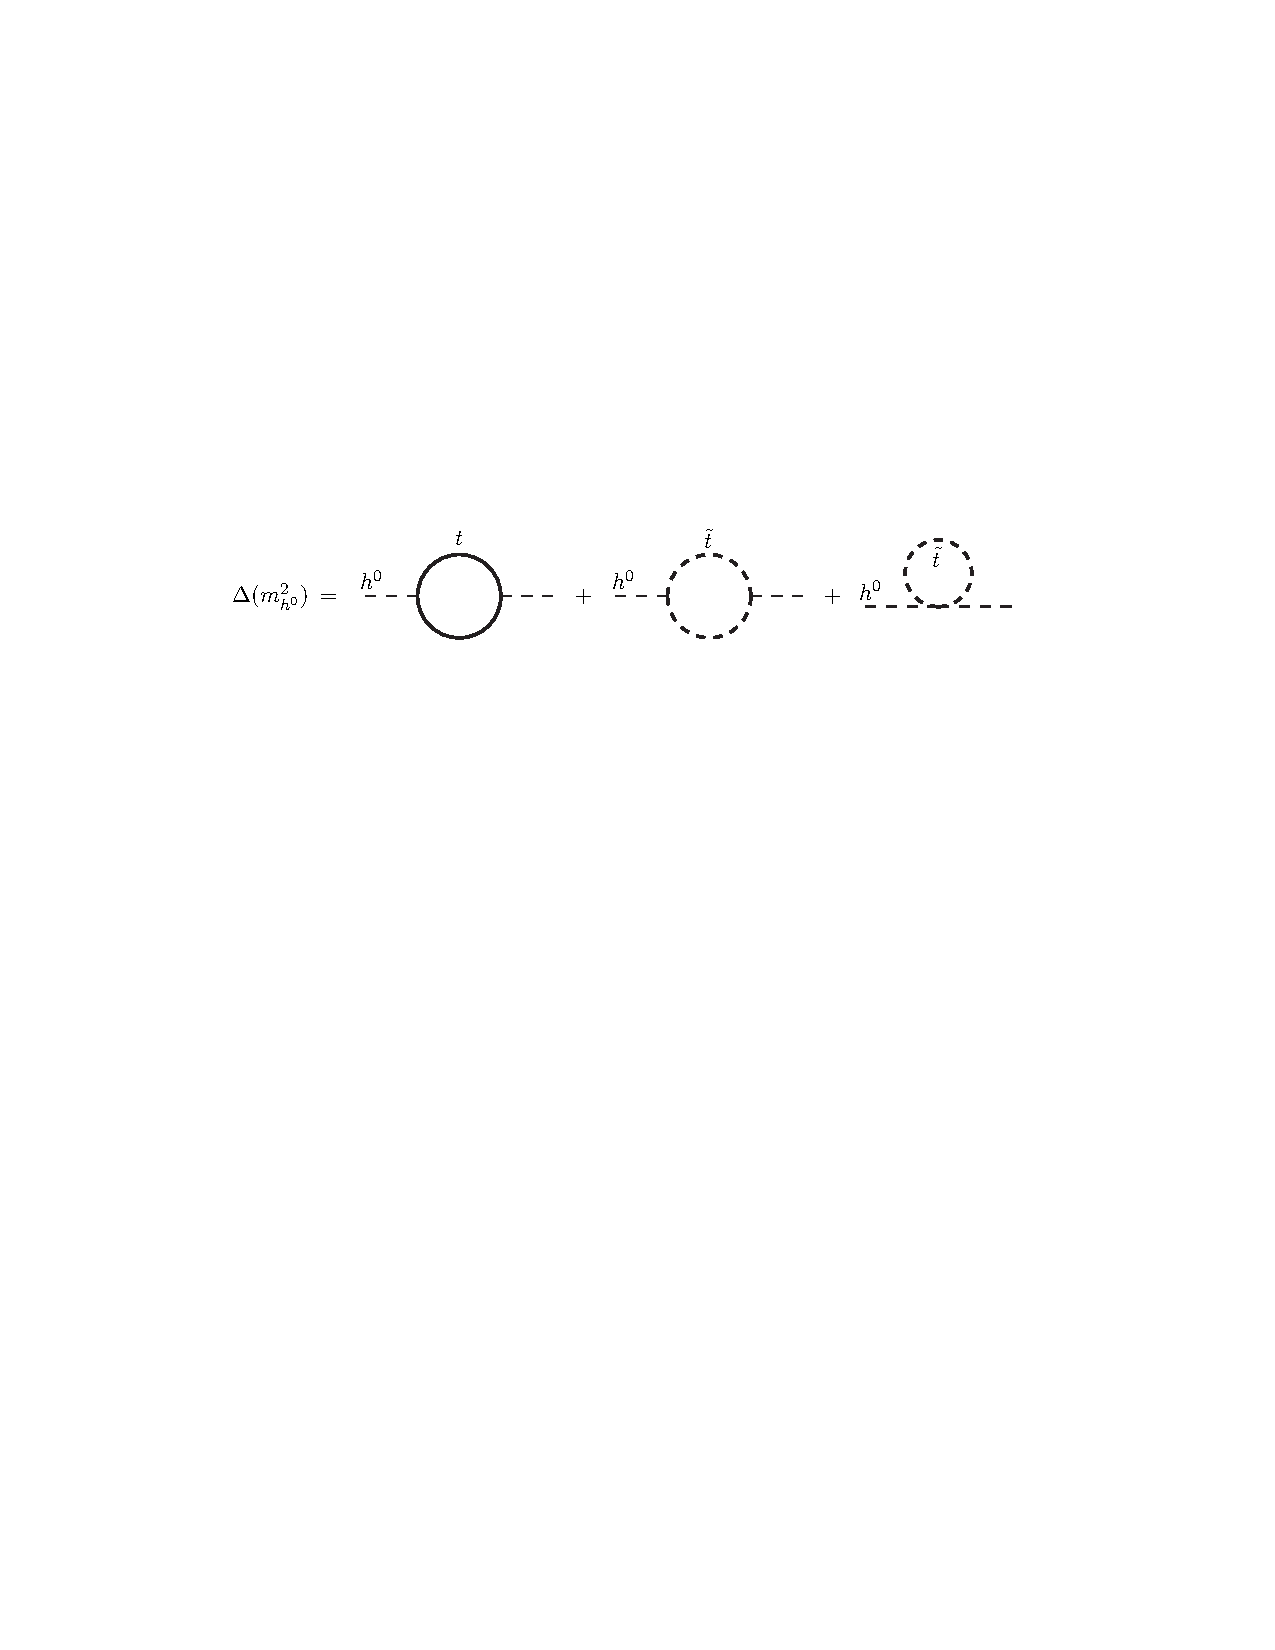
\includegraphics[width=0.7\textwidth]{higgs-loop-cancel}
\label{fig:susy:higgs-loop-cancel}
\caption{A schematic diagram of the top quark and stop squark loops involved in renormalizing the Higgs mass in SUSY, from~\cite{Martin1997}.}
\end{figure}

%%%%%%%%%%%%%%%%  

In SUSY, the top is not the only particle which contributes heavily to the mass renormalization of the Higgs: the \textit{stop squarks}, because of their supersymmetry with top quarks, have the exact same coupling to the Higgs. The complete set of diagrams that contibute is displayed in Figure~\ref{fig:susy:higgs-loop-cancel}. The solution here lies in the fact that boson and fermion loops come in with an opposite sign: this rule is often referred to as the ``Fermi minus sign'', and it means that the stop quark and top quark loops go in opposite directions. Both of these are formally infinite, but can cancel up a value proportional to the mass of stops and tops: \cite{Martin1997}
%
\begin{equation}
\Delta(m_{h^0}^2) = \frac{3}{4\pi^2} \cos^2 \alpha y_t^2 m_t^2 \ln \left( m_{\tilde{t}_1} m_{\tilde{t}_2} \right),
\end{equation}
%
where $\alpha$ is a mixing angle related to the SUSY Higgs sector, and $y_t$ is the top Yukawa coupling.

The corrections are finite, and naturalness was restored--- and all we needed was a light stop squark~\cite{Dimopoulos:1981zb,Witten:1981nf,Dine:1981za,Dimopoulos:1981au,Sakai:1981gr,Kaul:1981hi}! Unfortunately, the situation is not quite so simple: the stop itself is a scalar and undergoes similar mass renormalization as the Higgs~\cite{natural}. In particular, the previously alluded to gluino, because of its color charge, couples especially strongly to the stop squark in this loop and dominates the mass renormalization. In particular, it pulls the mass of the stop squark \textit{up} as~\cite{natural}:
%
\begin{equation}
\partial_t m_{\tilde{t}}^2 = - \frac{8\alpha_s}{3\pi} M_3^2
\end{equation}
%
where $M_3$ is the mass of the gluino in the IR and the $t = \log \mu$. This consequence of this, after solving the renormalization group equations, are that the stop should have about half the mass of the gluino--- or else very specific tree-level initial values are required keep the stop mass lighter. Thus, in addition to light stops, our theory should also have light gluinos~\cite{natural}.

The story is not completely finished yet--- the Higgsinos also contribute, since the Higgs and the Higgsinos should have similar masses. The Higgsinos form a component of the Neutralino, so this means that the \lsp should not be too heavy either~\cite{natural}.


\subsubsection{Model Building, and Simplified Models}

Our efforts to impose naturalness with SUSY have run into a few complications, but the situation is still rather simple. Our requirements for natural, un-tuned models are:
%
\begin{itemize}
\item Light stops in order to cancel the divergent top loops in the Higgs mass renormalization
\item Light gluinos because of the radiative corrections to the stop mass
\item Light neutralinos because of the relationship between the Higgs and Higgsinos
\end{itemize}
%
What about the other SUSY particles--- the squarks, the sleptons, and so forth? A full SUSY model will likely have them, but for the sake of experimental analyses, a \textit{simplified model} approach can be adopted~\cite{simplified}. In these models, a minimal set of particles related to a particular observable signature is kept at low mass; all the other particles are set to high masses, and are effectively integrated out using an Effective Field Theory approach. We can use this philosophy in considering our minimal set of required particles: others can exist, but have a much smaller effect on the physics of naturalness, and so we essentially ignore them.


An important question remains for the model: how will the new physics actually be produced? It is possible, for example, to directly produce pairs of \lsp's and search for such a signature immediately, but another attractive option goes back to the gauge couplings of the squarks and gluino. In particular, the LHC is a hadron collider and therefore is colliding quarks and gluons: production of particles which strongly couple to quarks and gluons is therefore expected to be enhanced. The \lsp has no such coupling, but the squarks do, and the gluino, because of its higher color charge, has an even larger coupling. Figure~\ref{fig:susy:multi_strong} shows the production cross-sections for gluions, squarks, and stops alone: the higher multiplicity of treating squarks inclusively (as well as $t$-channel production which is possible for the light flavors) raises their production over that of stops alone, but the gluinos have the highest cross-section of all. 

%%%%%%%%%%%%%%%%

\begin{figure}
\centering
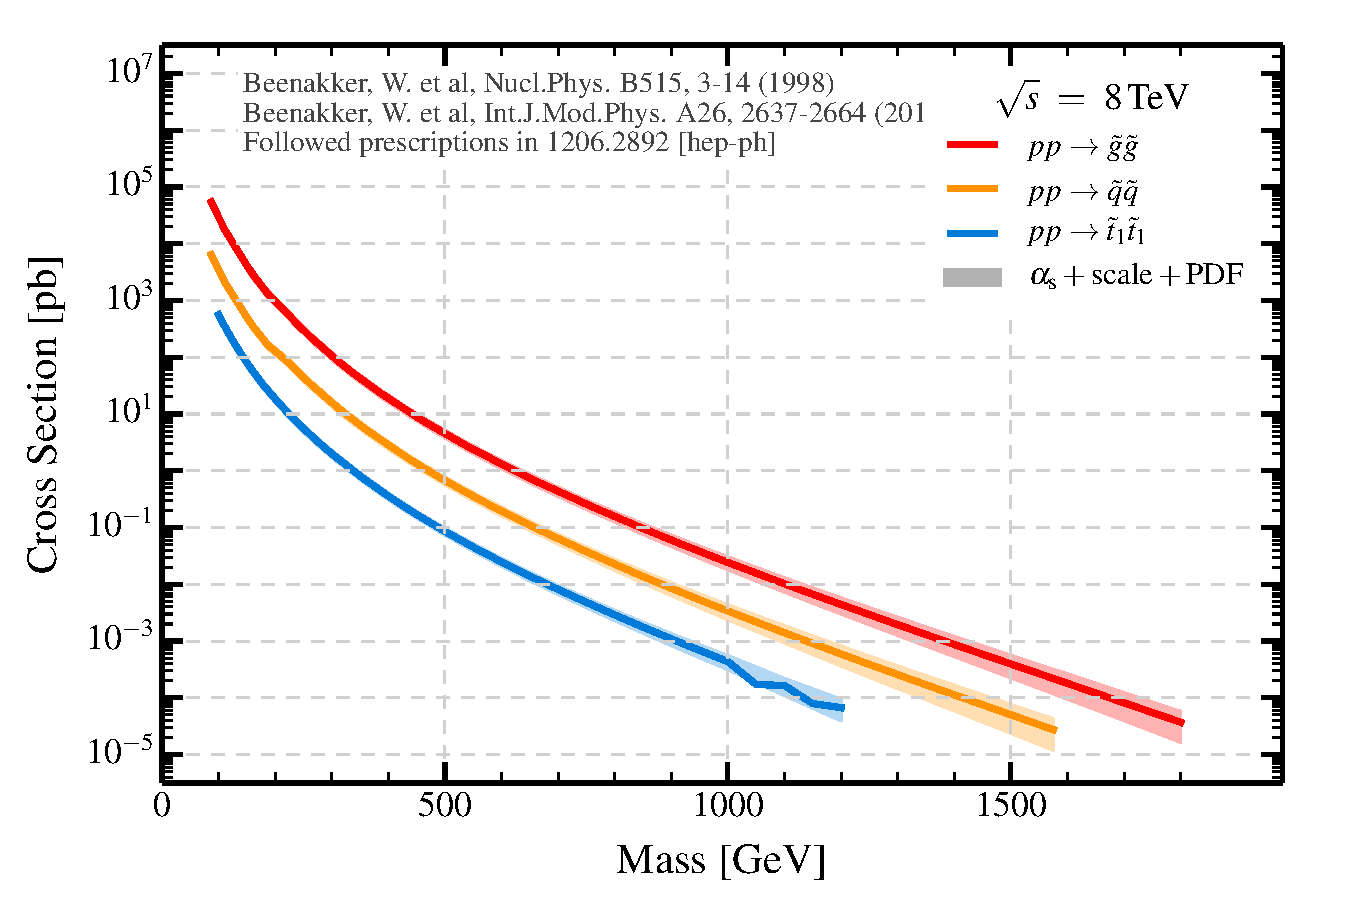
\includegraphics[width=0.7\textwidth]{multi_strong-2.pdf}
\label{fig:susy:multi_strong}
\caption{The production cross-section of various strongly interacting SUSY particles. From ATLAS SUSY group.}
\end{figure}

%%%%%%%%%%%%%%%%  

How do all of these requirements fit together? Figure~\ref{fig:susy:gtt} gives an example of the Feynman diagrams which combine all of these various requirements. Gluino pair production is used as the production mode, as it has the largest cross-section. Stops are the lightest squarks, and are either heavier than the gluino (in which case the decay to the \lsp is off-shell), or lighter than the gluino. The final states are filled with top quarks and large missing energy from the \lsp. Figure~\ref{fig:susy:spectra} shows an example of possible masses of particles in these models.


%%%%%%%%%%%%%%%%%%%%%

\begin{figure}
\centering
\subfigure[Off-shell stop]{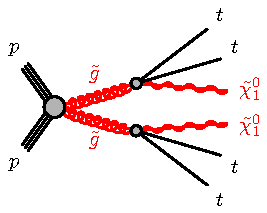
\includegraphics[width=0.45\textwidth]{gogo-ttttN1N1.pdf}}
\subfigure[On-shell stop]{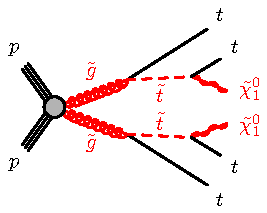
\includegraphics[width=0.45\textwidth]{gogo-ttttN1N1-stst.pdf}}
\label{fig:susy:gtt}
\caption{Feynman diagrams for natural SUSY processes at the LHC, in the case of off-shell stops and on-shell stops.}
\end{figure}

%%%%%%%%%%%%%%%%%%%%%


%%%%%%%%%%%%%%%%

\begin{figure}
\centering
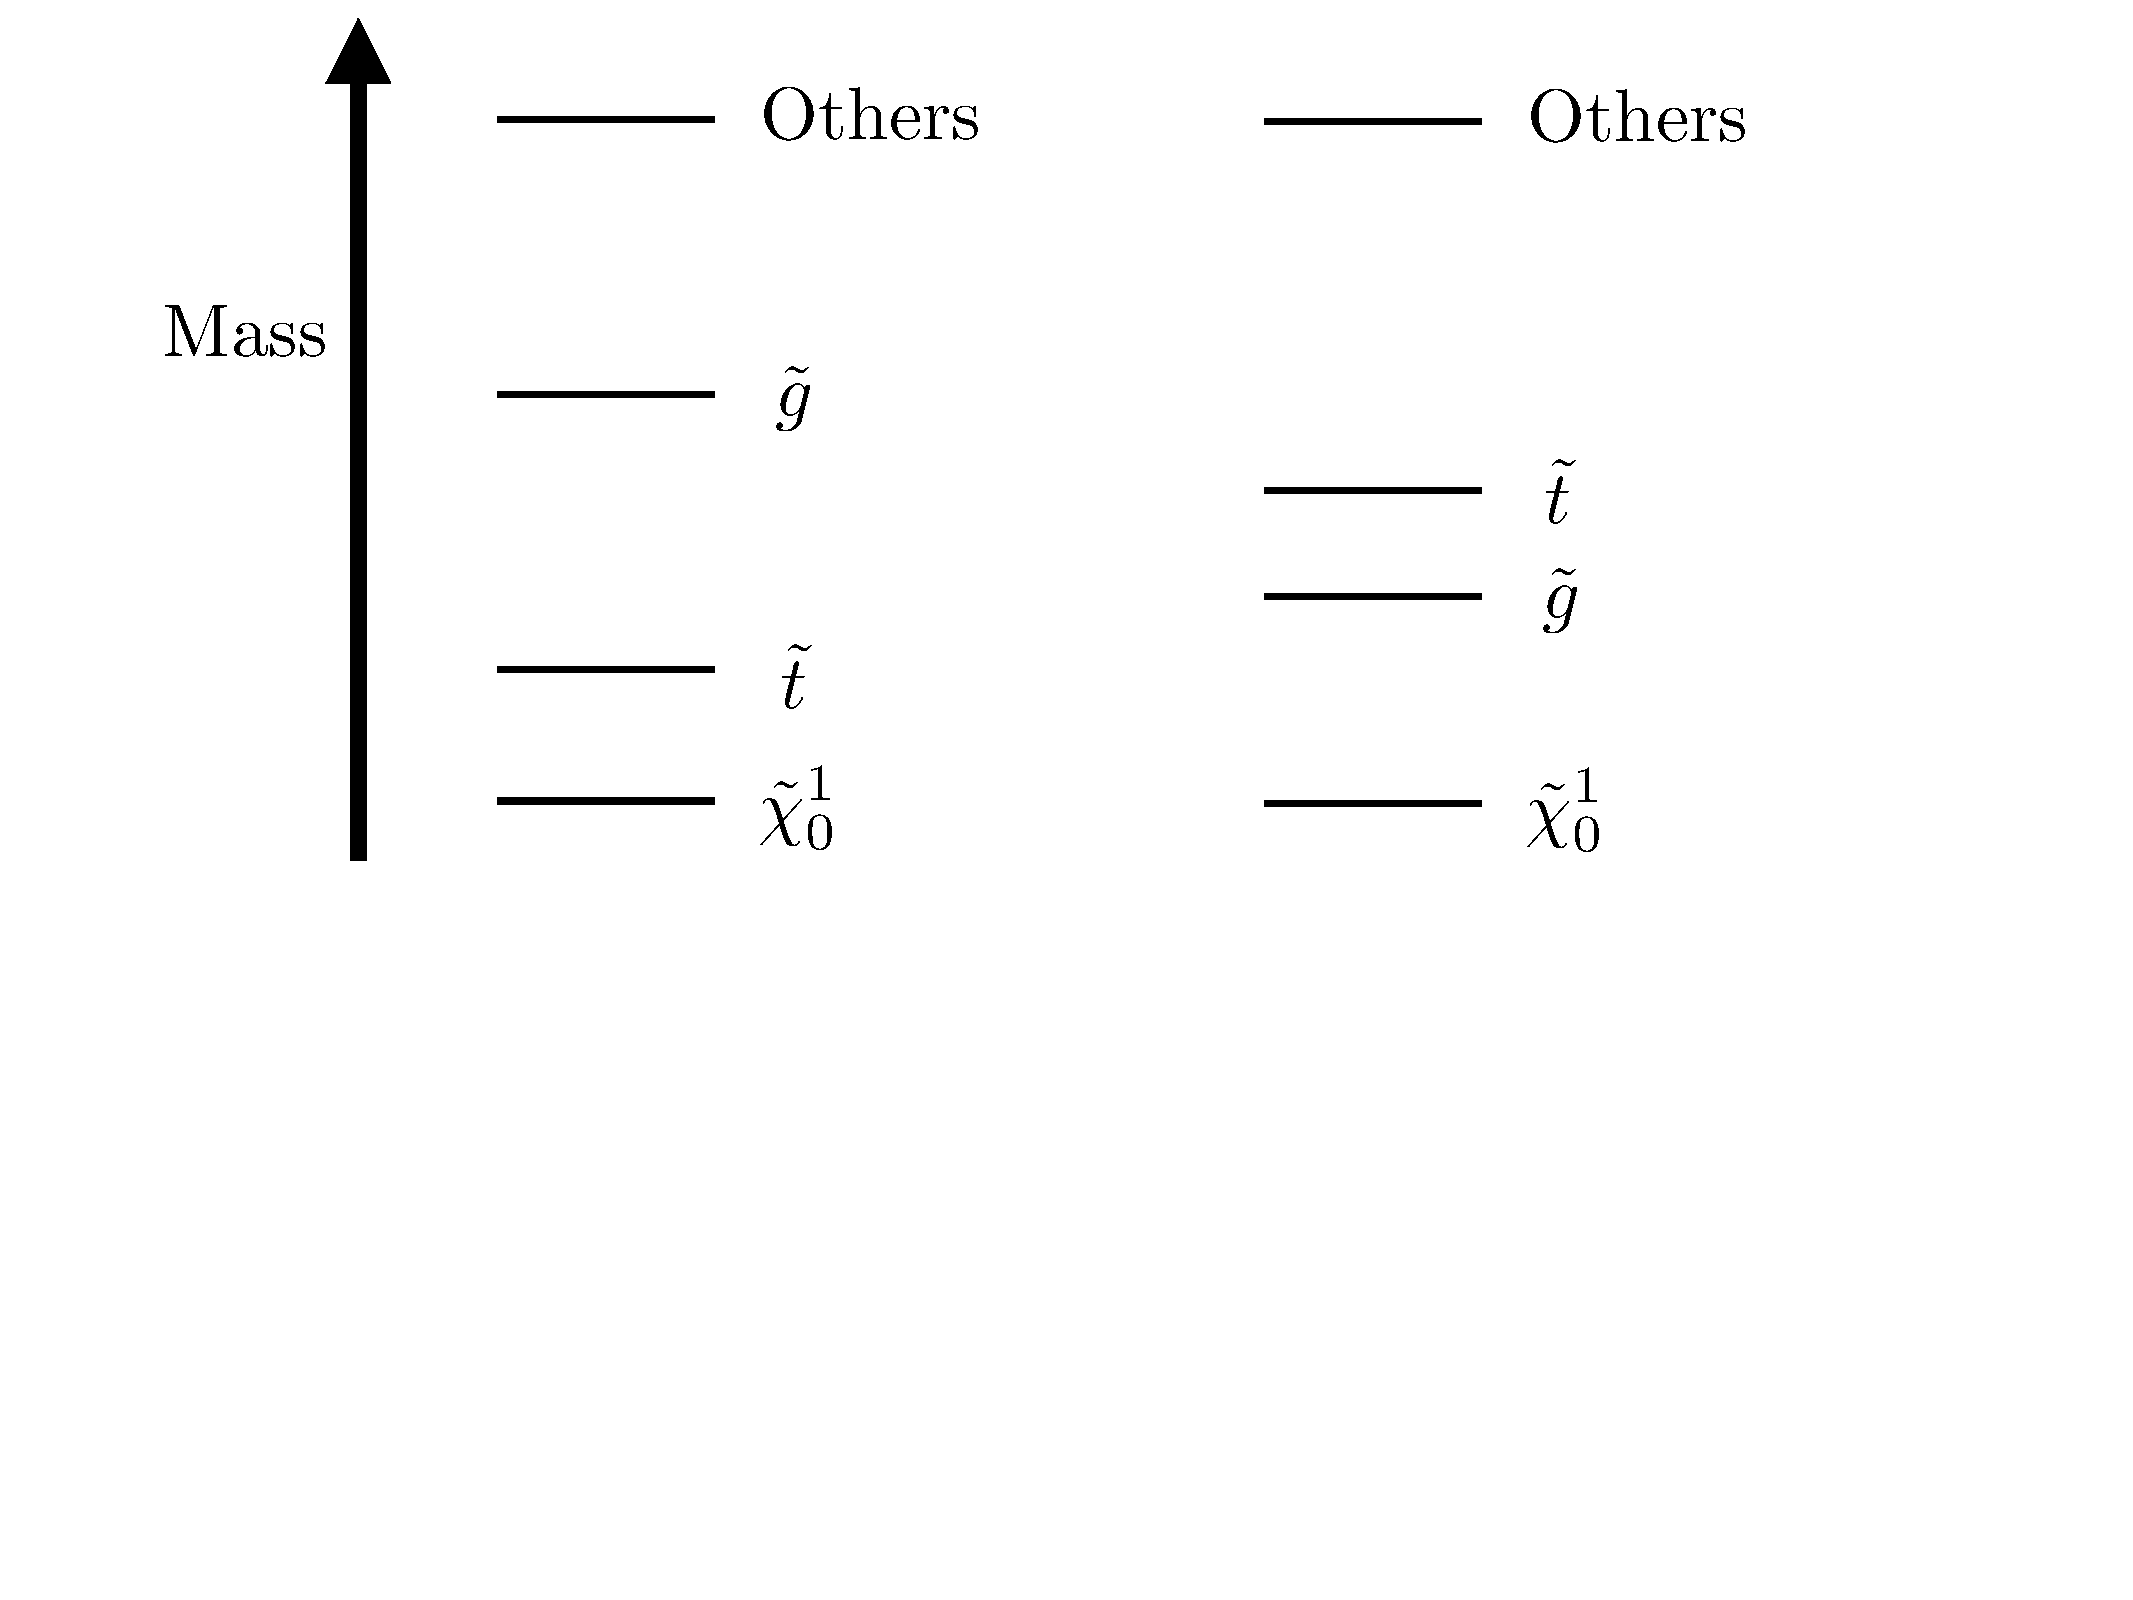
\includegraphics[width=0.7\textwidth]{spectra.pdf}
\label{fig:susy:spectra}
\caption{Examples of SUSY simplified model spectra which satisfy the requirements of naturalness.}
\end{figure}

%%%%%%%%%%%%%%%%  

%spectra

%diagram from martin

%gluino suck

\subsection{Coupling Unification}

% plot from hitoshi; quote some of the changes to \beta functions

It turns out that SUSY fixes more than just the naturalness issue of the Standard Model: it also changes the evolution of the coupling constants to suggest that all the forces unify, as seen in Figure~\ref{fig:susy:couplings_mssm}~\cite{susypheno,SUSYUnification}. Is this meaningful, or a coincidence? It is hard to tell, since the unification scale of $\mu \approx 10^{16}$~GeV is well outside experimental access.

%%%%%%%%%%%%%%%%

\begin{figure}
\centering
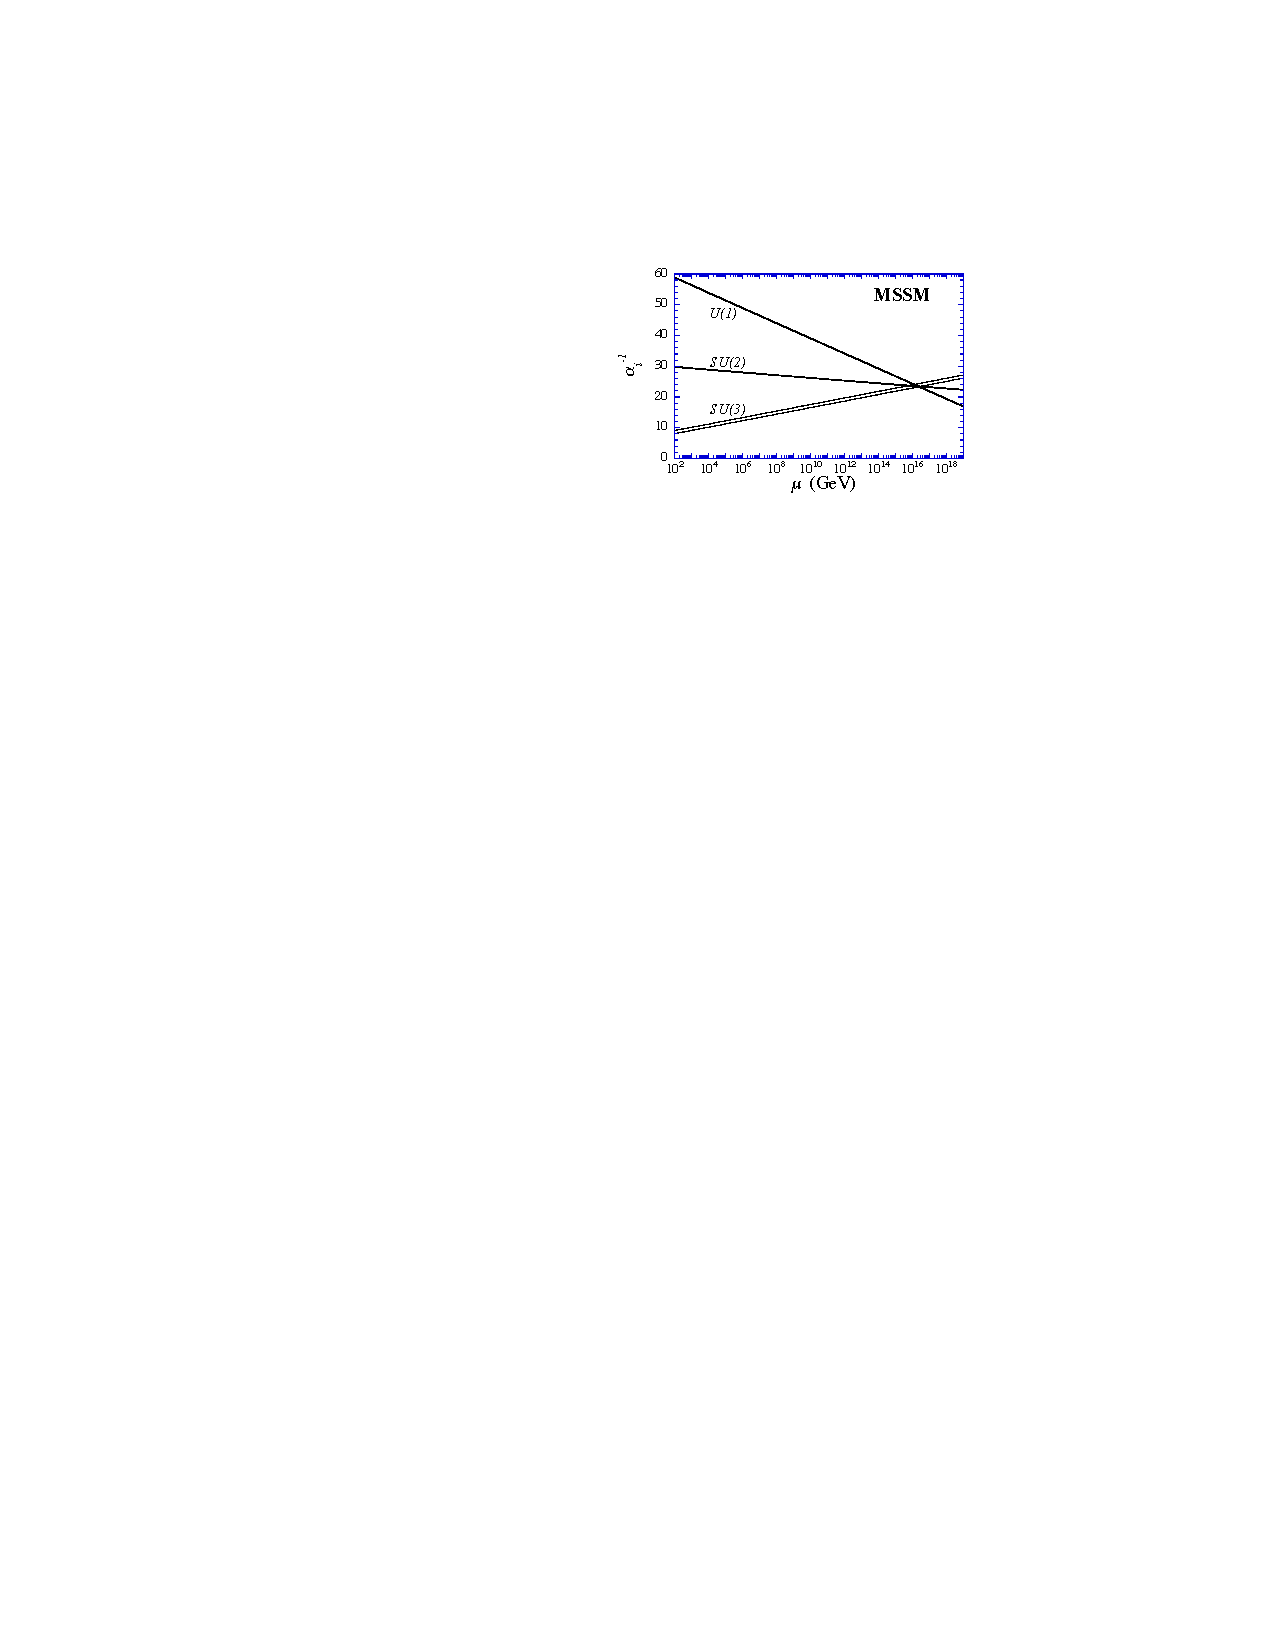
\includegraphics[width=0.7\textwidth]{couplings_mssm.pdf}
\label{fig:susy:couplings_mssm}
\caption{The evolution of the strength of the coupling constants of the three symmetry groups of the SM, in the MSSM. They clearly all meet at one point, suggesting that a large symmetry group would be able to unify them at the $\mu = 10^{16}$~GeV mass scale. Figure from \cite{susypheno}.}
\end{figure}

%%%%%%%%%%%%%%%%  

\subsection{Dark Matter}

Finally, we turn to the subject of the missing matter in the universe: dark matter. In our earlier construction of the model, we had assumped the presence of $R$-parity, which guaranteed the stability of the LSP\footnote{It is easy to see what this guarantees LSP stability, as it requires all interactions are guaranteed to couple an even number of supersymmetric particles and one SM particle. This means that moving down a mass cascade, a heavy SUSY particle can decay to lighter SUSY particles and SM particles, but the lightest is stable.}. For reasons of naturalness, we have already required a light neutralino \lsp, but this particle has other attractive properties. It is electromagnetically neutral, and interacts only via the weak nuclear force: this makes it a perfect candidate to be the Weakly Interactive Massive Particle (WIMP) preferred by large-scale galactic simulations~\cite{Goldberg:1983nd,Ellis:1983ew,Jungman}.

Since the \lsp is expected to be stable, there should be a number of them left over from production in the Big Bang. The density is defined by the rates of annihilation ($\chi\overline{\chi} \rightarrow l \overline{l}$) and production ($l\overline{l}\rightarrow \chi\overline{\chi}$. As the universe cools, eventually the annihilation rate falls below that of the expansion rate of the universe, thereby freezing out the mechanisms which maintain thermal equilibrium and leaving a ``relic'' cosmological abundance \cite{Jungman}.The correct description for the number density $n_\chi(t)$ out of equilibrium is given by the Boltzmann equation:
\begin{align}
  \df{n_\chi}{t} + 3 H n_\chi = - \langle \s_A \nu \rangle [(n_\chi)^2 - (n_\chi^\mathrm{equi})^2]\label{eqn:boltz}
\end{align}
where $H=\dot{a}/a$ is the Hubble expansion rate, $\langle\sigma_a \nu\rangle$ is the thermally averaged cross-section, $a$ is the scale factor, and $n_\chi^\mathrm{equi}$ is the thermal equilibrium distribution, given by either the Fermi-Dirac or Bose-Einstein distribution. The second term on the left corresponds to the expansion of the universe; number changing interactions provide the terms on the right hand side, as the first term accounts for depletion from annihilation and the second comes from creation from inverse annihilation. 

Solving this equation leads to a prediction for the thermal relic of this new particle with mass near the electroweak scale. The ``Dark Matter Miracle'', is that an appropriate value for the annihilation cross section, $\langle \sigma_A \nu \rangle \sim \alpha^2 (100~\mathrm{GeV})\sim 10^{-25}~\mathrm{cm}^3\mathrm{s}^{-1}$, is predicted just based on the idea of this new particle existing at the electroweak scale. This value gives the approximately measured density of dark matter as seen by measurements (rotation curves, etc.) and simulation (large-scale structure). 

SUSY provides a candidate a compelling candidate for WIMP Dark Matter with the neutralino \lsp, which we have already required to have a mass near the electroweak breaking scale for the sake of naturalness. Another hole in the Standard Model is thus miraculously solved by SUSY--- it is clear why this theory has gathered so much interest from theorists and experimentalists over the years.

\section{The Status of SUSY after LHC Run 1}
\label{chapter:susy:status}

%stop and gluino limits
With Run 1 of the LHC coming to a close, an extremely detailed program  of searches for SUSY at the ATLAS detector has been finished~\cite{Atlassusy1lepton,susyoleptons,Aad:2011ks,SUSYZeroLep2011,SUSYOnelep2011,SUSYJetMult2011,SUSYTwoLep2011,SUSYStopGluino2010,Aad:2013wta,Aad:2014lra}. Unfortunately, none of these analyses have seen any excesses beyond the expectation of SM production\footnote{With the exception of one $3\sigma$ excess in \cite{Aad:2015wqa}, though perhaps one fluctuation in such a large dataset is expected.}. Figure~\ref{fig:susy:limits} shows the limits on production in two particularly relevant sets of analyses: the search for direct production of stop quarks which decay to neutralinos, and the production of gluinos which decay through stop quarks to neutralinos. These are exactly the simplified models we have been earlier motivated by with our concerns about naturalness, but with no excesses in sight in these channels, even SUSY starts to require significant artificial tuning.



\begin{figure}[htbp]
  \centering
    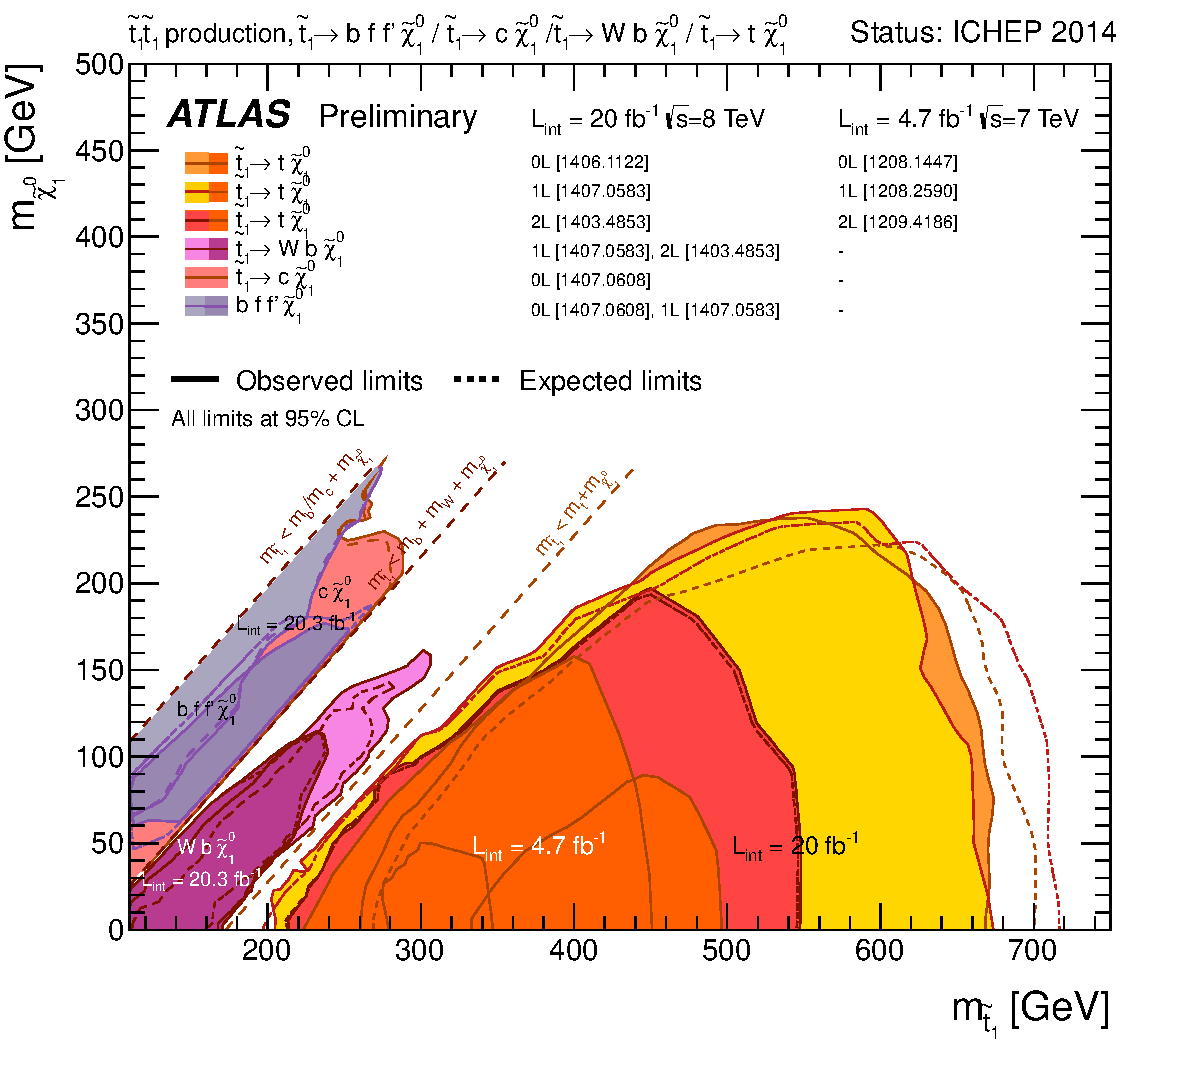
\includegraphics[width=0.45\textwidth]{ATLAS_SUSY_Stop_tLSP}
    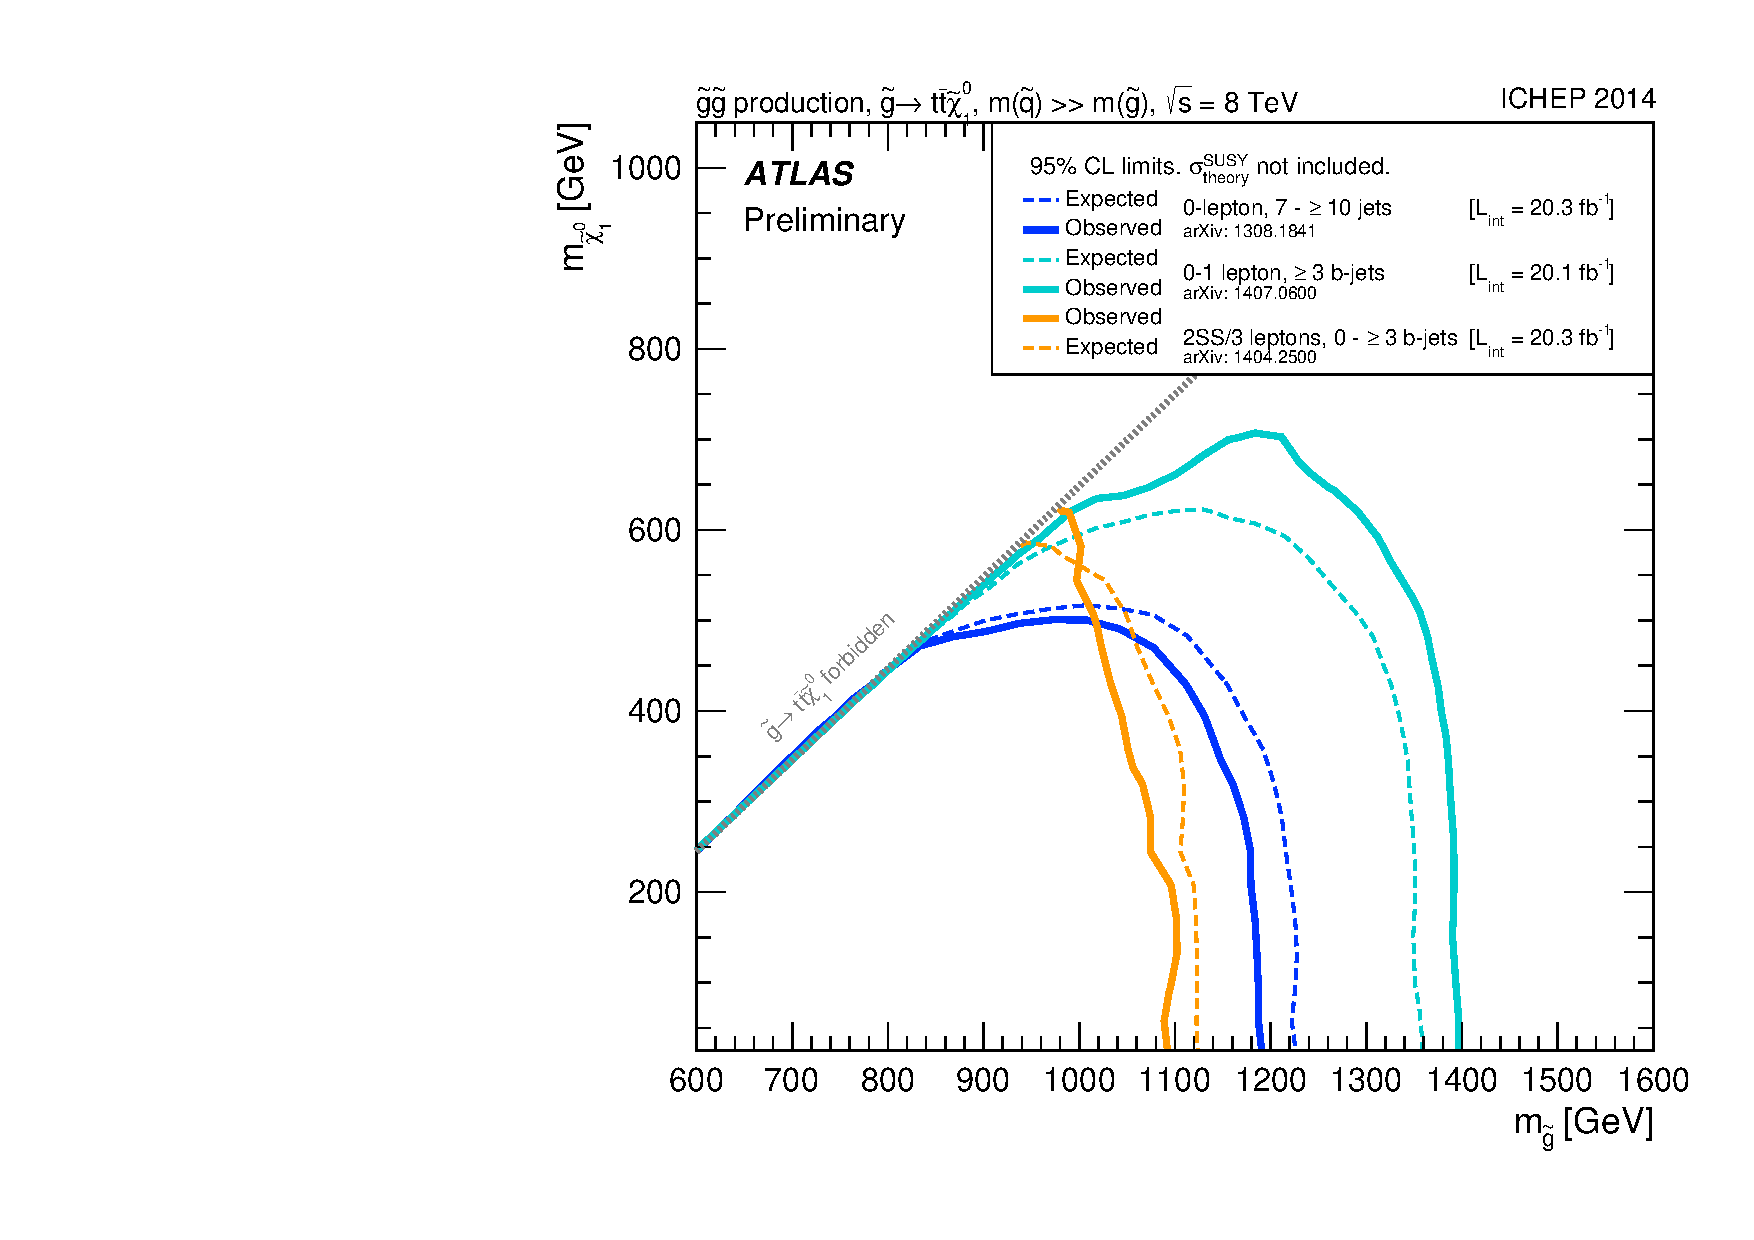
\includegraphics[width=0.45\textwidth]{ATLAS_SUSY_Gtt}
  \caption{The limits on SUSY particles in the $\tilde{t}-\lsp$ (left) and $\tilde{g}-\lsp$ (right, with $\tilde{t}$ as lightest squarks). Stops are excluded to 700 GeV, and gluinos to 1.4 TeV, severely stressing the hopes of naturalness.}
  \label{fig:susy:limits}
\end{figure}


\subsection{Assumptions}

A relevant question to ask at this point is whether there is an underlying assumption in the experimental searches which is crippling our search for SUSY. Is one of our theoretical requirements biasing our approach to searching for new physics?

Consider the requirement of the stop quark being light--- while the searches in Figure~\ref{fig:susy:limits} require the experimental signatures related to stops (i.e., top quarks in the final state), many other searches exists which assume only light flavor squarks are dominantly produced. These searches too see no hints of new physics.

This leads us to the assumption of the light \lsp, and its stability. Figure~\ref{fig:susy:meff} shows an example of one search and the variables used in it. This variable, $m_{\rm eff}$, is composed as the sum of \met and \Ht in an event: because of the stability and weakly-interacting nature of the \lsp, it does not interact with the detector and therefore appears as missing energy. Almost every ATLAS SUSY search makes this assumption, and uses variables related to the \met to construct their searches. 
 
%%%%%%%%%%%%%%%%

\begin{figure}
\centering
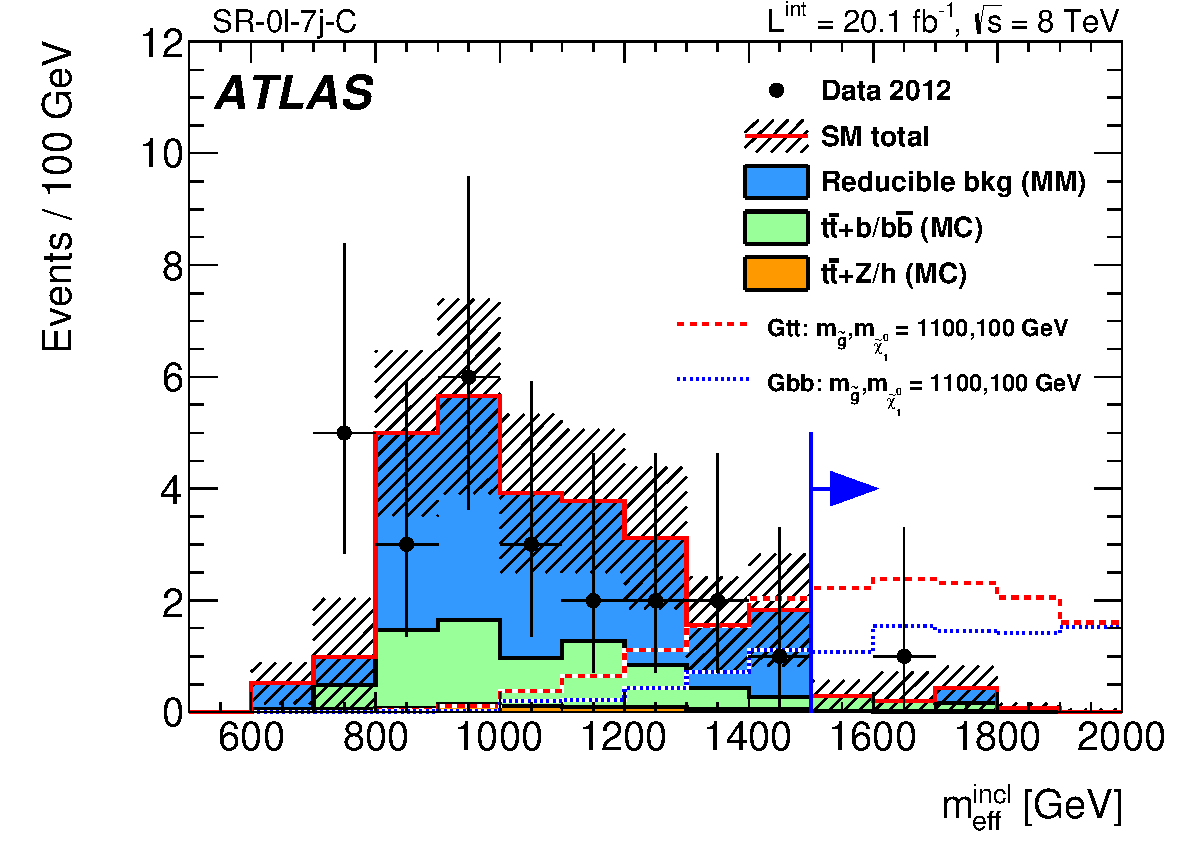
\includegraphics[width=0.7\textwidth]{meff.pdf}
\label{fig:susy:meff}
\caption{The $m_{eff}$, or the sum of \met and \Ht in an event, used in a search for gluinos decaying through stop squarks. From \cite{Aad:2014lra}.}
\end{figure}

%%%%%%%%%%%%%%%%  

This assumption motivates us to reconsider the statement of $R$-parity we began with. Is it possible to remove this symmetry from the model, thereby allowing the \lsp to decay to SM particles? Are there any other experimental limits that prevent this? 

\section{$R$-Parity, and How to Violate It}
\label{chapter:susy:r}
		 % from martin
Earlier in Section~\ref{chapter:susy:susy:developing}, we assumed the presence of a $R$-parity, defined as $R_p = (-1)^{3(B-L)+2S}$. This eliminated the following terms from the potential~\cite{dreinerRPV}:
%
%---------------------
  \begin{eqnarray} 
    \Wrpv &= \frac{1}{2} \lamijk L_{i}L_{j}\Ebar_{k} + \lampijk L_{i}Q_{j}\Dbar_{k} +  \nonumber \\
       & \quad \frac{1}{2}\lamppijk\Ubar_{i}\Dbar_{j}\Dbar_{k} + \kappa_iL_{i}H_{2},
    \label{eqn:rpvandudd:wrpv}
  \end{eqnarray} 
%---------------------

\noindent where $i,j,k=1,2,3$ are generation indices (which may be ommitted from the discussion below if the statements do not depend on generation). The last term, referred as the the bilinear coupling, can be removed from the theory by a rotation of the $L$ and $H$ superfields, and so is commonly ignored~\cite{dreinerRPV}. The first three trilinear terms, with Yukawa couplings for each term are given by \lam, \lamp, and \lampp, are generally non-trivial. The particle content with these new terms is identical to that of $R$-parity conserving (RPC) models, but the $R$-parity violating (RPV) terms add new interactions.

The structure of these interactions couples one supersymmetric particle together with two SM particles. This has many experimental consequences, not only in the signatures in colliders, but also in the interactions of SM particles at low energy. Interactions, such as the one in Figure~\ref{fig:susy:rpv_proton} in which an off-shell squark couples a two quarks to a lepton and a quark, can occur: though suppressed by the mass of the squark in the mediator, such an interaction should occur fairly frequently if $\lamp > 0$ and $\lampp > 0$. In particular, purely on dimensional grounds we can estimate the decay rate of the proton based on this diagram as~\cite{dreinerRPV}:
%
\begin{equation}
\Gamma(P\rightarrow e^+ \pi^0) \approx \frac{\lambda_{11k}^{'2} \lambda_{11k}^{''2}}{16\pi^2 m^4_{\tilde{d}_k}} M_\mathrm{proton}^5
\end{equation} 
%
A host of detectors, starting with the IMB~\cite{Gajewski:1989gh} and Kamiokande~\cite{Regis:2012sn} detectors, were built to study the proton decays predicted by RPV and other theories (primarily Grand Unified Theories which introduced similar operators and lead to $e^+ \pi^0$ final states). These detectors were filled with huge amounts of water--- with $O(10^{31})$ protons--- and were lined with photo-multiplier tubes which could detect the Cerenkov radiation which would have been emitted by the electrons and pions if they were produced in a proton decay. No events were observed in any of these detectors or their upgrades or successors, setting limits on the proton lifetime at $\tau(P\rightarrow e^+ \pi^0) > 10^{32}$ years. Thus, the simplest models of RPV SUSY with large couplings to all $\lambda$ modes are clearly excluded; these are often recast into the RPV space as~\cite{PhysRevD47279}:
%
\begin{eqnarray}
  \lamp_{11k}\cdot\lampp_{11k}\; \lsim\; 10^{-23} \left( \frac{{\msquark}} {100~\gev} \right)^2,
  \label{eqn:rpvandudd:protondecay}
\end{eqnarray}
%
where \msquark is the typical squark mass. 

\begin{figure}
\centering
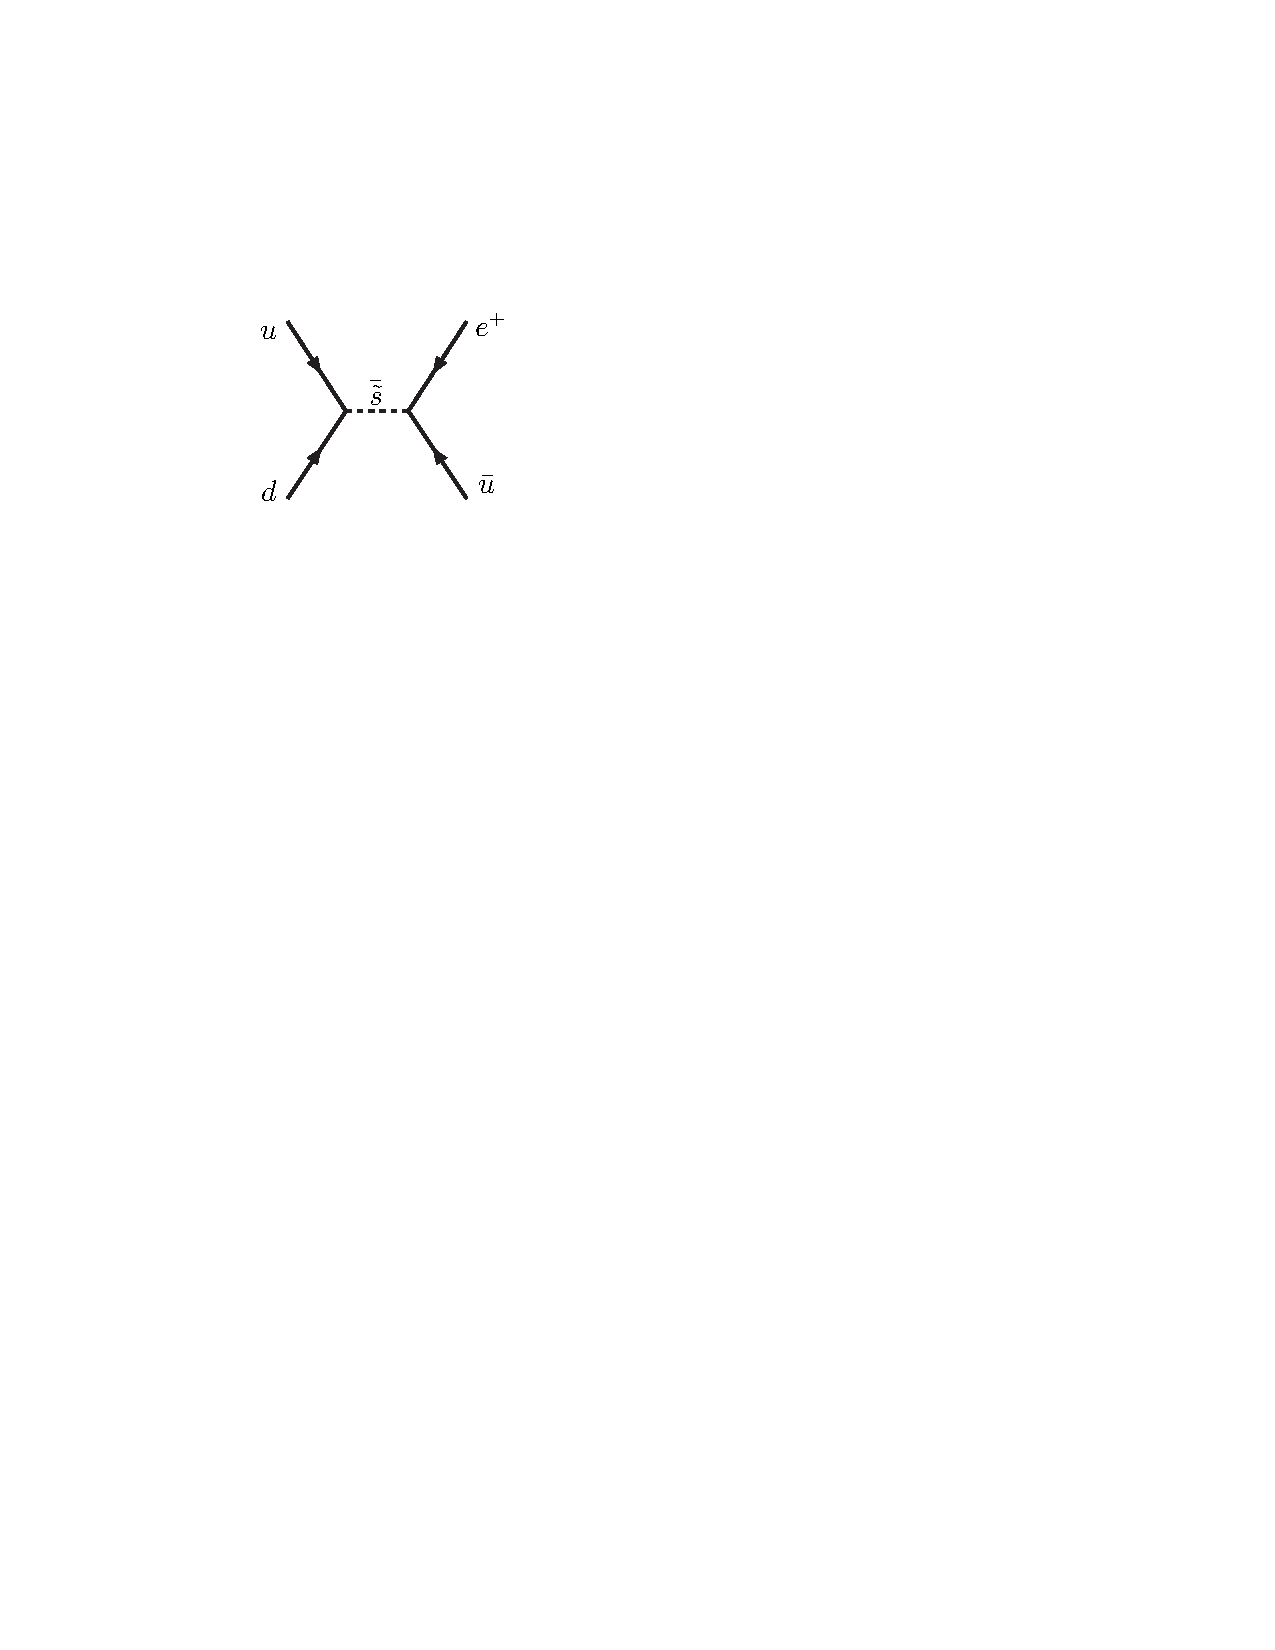
\includegraphics[width=0.5\textwidth]{rpv_proton.pdf}
\label{fig:susy:rpv_proton}
\caption{One example of a diagram which contributes to rapid proton decay in RPV models with $\lampp > 0$ and $\lamp > 0$.}
\end{figure}

This is obviously a very strong restriction, and thus most modern RPV models impose an \textit{ad hoc} condition to require the proton to be stable. This is mostly easily done by requiring that at least one of \lamp or \lampp be exactly equal to zero. If the \lampp term is zero, then the proton stability is clearly preserved, as the off-shell squark in Figure~\ref{fig:susy:rpv_proton} is not able to occur. If $\lam = 0$ and $\lamp = 0$, then $\lampp > 0$ only if the LSP has mass greater than the proton: otherwise, the off-shell squark could decay to an LSP and a quark and the proton could still decay. This is usually a not very strong restriction, however, as the LSP can easily have mass $> 1$~GeV.

The collider signatures of such models are obviously extremely different from RPC scenarios, even if the particle spectrum remains identical. If $\lam > 0$ or $\lamp > 0$, the final states will include leptons instead of the large missing energy tradtionally attributed to the \lsp. Similarly, if $\lampp > 0$, the final states will include many more quarks instead of missing energy. The decay goes through an offshell squark (or slepton), as $\lsp \rightarrow \tilde{q} q$, $\tilde{q}\rightarrow q q$. These signatures are potentially not explored by current LHC analyses, which almost uniformly rely on high missing energy signatures. Figure~\ref{fig:susy:rpv_diagrams} shows several examples of potential models at the LHC: gluino and squark pair production normally has final states dominated with only quarks and missing energy, but these models show the possibility of extra leptons or jets.

% %
% \noindent where \msquark is the typical squark mass. As a result, even when considering this more generic form of the \SUSY superpotential by including \Wrpv, it is still necessary to impose an \textit{ad hoc}, albeit experimentally motivated, symmetry to protect the proton from decay. It is generally necessary that at least one of \lam, \lamp, \lampp be exactly equal to zero. Consequently, it is common to consider each term in Equation~\ref{eqn:rpvandudd:wrpv} independently. In the case of nonzero \lam and \lamp, the typical signature involves leptons in the final state. However, for $\lamppijk \neq 0$, the final state is characterized by jets, either from direct gluino decay or from the cascade decay of the gluino to the lightest neutralino (\ninoone), as also considered here. Because of the structure of Equation~\ref{eqn:rpvandudd:wrpv}, scenarios in which only $\lamppijk \neq 0$ are often referred to as UDD scenarios.


% Current indirect experimental constraints~\cite{Allanach:1999ic} on the sizes of each of the UDD couplings \lamppijk from sources other than proton decay are valid primarily for low squark masses, as suggested by Equation~\ref{eqn:rpvandudd:protondecay}. Those limits are driven by double nucleon decay~\cite{Sher:1994sp} (for $\lampp_{112}$), neutron oscillations~\cite{Zwirner1983103} (for $\lampp_{113}$), and $Z$ boson branching ratios~\cite{Bhattacharyya:1997vv}.

%%%%%%%%%%%%%%%%%%%%%

\begin{figure}
\centering
\subfigure[$\lam> 0$]{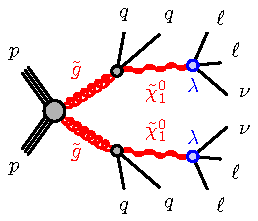
\includegraphics[width=0.45\textwidth]{gogo-qqqqllllvv-RPV.pdf}}
\subfigure[$\lamp > 0$]{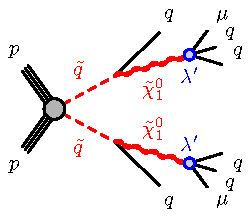
\includegraphics[width=0.45\textwidth]{sqsq-qqlqql-N1N1-RPV.pdf}}\\
\subfigure[$\lampp > 0$]{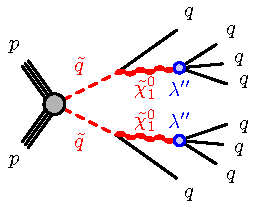
\includegraphics[width=0.45\textwidth]{sqsq-4q4q-RPV.pdf}}
\label{fig:susy:rpv_diagrams}
\caption{Feynman diagrams for several RPV processes at the LHC, each with a different $\lambda$ operator set to $>0$.}
\end{figure}

%%%%%%%%%%%%%%%%%%%%%

It should be noted that the lifetime of the \lsp is proportional to the $\lambda$ terms squared, and inversely proportional to the mass of the squark to the fourth. For particular combinations of these values, it is thus possible for the \lsp to have a significant lifetime and therefore to proceed through the detector some distance before decaying. This can lead to a spectacular displaced signature, which again would be missed by most SUSY searches~\cite{Graham:2012th}. 


\section{Conclusions}

In summary, SUSY is a strongly compelling theory of BSM physics. Its solution to the naturalness problem--- the introduction of a boson/fermion symmetry--- is effective and simple. It furthermore allows for the unification of forces at high energy. And finally, it produces a miraculous dark matter candidate in the form of the \lsp.

Unfortunately, given the results from the first run of the LHC, it is time to reconsider whether we can have all three miracles at once. The least explored space of possibilities exist in the realm of $R$-parity violating models, which have been largely unexplored because of the difficult signal discrimination and background estimation. Chapter~\ref{chapter:search} presents an innovative new search for exactly such models where $\lampp > 0$: the experimental issues are tackled with the aid of the tools of jet substructure developed in Chapter~\ref{chapter:jets-and-substructure}.